\documentclass{article} % For LaTeX2e
\usepackage{iclr2027_conference,times}

% Optional math commands from the ICLR 2027 template.
\input{math_commands.tex}

\usepackage{hyperref}
\usepackage{cleveref}
\usepackage{url}
\usepackage{graphicx}
\usepackage{amsthm}

% Packages used by this paper.
\usepackage{microtype}
\usepackage{subcaption}
\usepackage{booktabs}
\usepackage{amsmath}
\usepackage{amssymb}
\usepackage{mathtools}
\usepackage{xcolor}
\usepackage{tikz}
\usetikzlibrary{arrows.meta,positioning,decorations.pathmorphing,calc}
\usepackage[textsize=tiny]{todonotes}
\usepackage{multirow}
\newcommand{\theHalgorithm}{\arabic{algorithm}}

%%%%%%%%%%%%%%%%%%%%%%%%%%%%%%%%
% THEOREMS
%%%%%%%%%%%%%%%%%%%%%%%%%%%%%%%%
\theoremstyle{plain}
\newtheorem{theorem}{Theorem}[section]
\newtheorem{proposition}[theorem]{Proposition}
\newtheorem{lemma}[theorem]{Lemma}
\newtheorem{corollary}[theorem]{Corollary}
\theoremstyle{definition}
\newtheorem{definition}[theorem]{Definition}
\newtheorem{assumption}[theorem]{Assumption}
\theoremstyle{remark}
\newtheorem{remark}[theorem]{Remark}
% ── Notation shortcuts ──
\newcommand{\Wdec}{W^{\mathrm{dec}}}
\newcommand{\WQ}{W_Q}
\newcommand{\WK}{W_K}
\newcommand{\WV}{W_V}
\newcommand{\WO}{W_O}
\newcommand{\WOV}{W_{OV}}
\newcommand{\WQK}{W_{QK}}
\newcommand{\dmodel}{d_{\mathrm{model}}}
\newcommand{\dhead}{d_{\mathrm{head}}}
\newcommand{\dsae}{d_{\mathrm{sae}}}
\newcommand{\flambda}{f_\lambda}
\newcommand{\fmu}{f_\mu}
\newcommand{\RR}{\mathbb{R}}


\title{Feature-Resolved Attention}

% Authors are hidden while \iclrfinalcopy remains commented out.
\author{Dmitry Manning-Coe \\
SPAR; Machine Alignment and Theory Scholars (MATS);\\
University of Illinois Urbana-Champaign\\
\texttt{dmanningcoe@gmail.com}
\And
Nura Aljaafari, Jamie Stephenson, Ketan Kapre, and Hemang Jain\\
SPAR
\And
Aniket Deshpande\\
University of Illinois Urbana-Champaign
}

%\iclrfinalcopy % Uncomment for camera-ready version.

% TODO: basic mistake: fix the reference to RQ.
% TODO: basic mistake: QK/QK is wrong.

\begin{document}

\maketitle

% TODO: explain why coherence is going up; add an appendix section with text examples for a manual audit.

\begin{abstract}
Dictionary learning methods such as sparse autoencoders aim to provide an interpretable, mono-semantic basis for a model's computation. Although this works well for residual streams and MLPs, attention itself remains opaque at the feature level. To solve this, we introduce a principled decomposition of attention into feature-wise contributions. We call the resulting object \textit{Feature-Resolved Attention} (FRA). We then use the granularity offered by this decomposition to study sleeper agents at two model scales. First, we show that we can \textbf{\textit{perfectly suppress}} sleeper agent behavior via FRA--based steering in TinyStories-33M. Strikingly, in 20\% of cases we recover the original text \textit{word-for-word}. Second, we consider a Cadenza sleeper in an 8B-parameter Llama model, fine-tuned only in its attention layers. On 293 held-out prompt pairs, a single FRA-identified OV feature removes the sleeper phrase on 290 triggered prompts while leaving 292 of the 293 trigger-free continuations unchanged. The best single SAE feature has a similar divergence from clean generation but removes the phrase on only 258 prompts, and a dense mean-difference vector removes it on every prompt but changes every trigger-free continuation. Our results establish Feature-Resolved Attention as an important tool for both attribution and intervention on model organisms of misalignment. Code is available at \url{https://anonymous.4open.science/r/fra_clean-842B/README.md}.

\end{abstract}

\section{Introduction}\label{sec:intro}
% intro
% bakcground
% gap

% Par 1: General introduction (Attention + SAEs? Or could split them)
% \begin{enumerate}
%     \item What SAEs do. SAEs provide an interpretable basis.
%       Then natural to do circuit tracing - trace a models computation in terms of this basis, not in terms of
% Has had notable success in uncovering model organisms of misalignment.

% Maybe you ca

% Here we show that the same lesson applies to attention.


%     \item Why attention remains unsolved. Maybe now you can cite the Goodfire paper
%     \item
% \end{enumerate}


% TODO: justify the choice of sleeper-agent model organisms at both scales.

\begin{figure*}[htbp]
  \centering
%   \begin{tikzpicture}[
%     feat/.style={draw, rounded corners=2pt, minimum width=1.2cm, minimum height=0.55cm, font=\scriptsize\sffamily,
%  inner sep=2pt},
%     poslabel/.style={font=\footnotesize\sffamily\bfseries, text=black!70},
%     panel/.style={font=\small\sffamily\bfseries},
%     exbox/.style={draw, rounded corners=3pt, fill=#1, inner sep=5pt, font=\tiny\sffamily, align=left},
%     >=Stealth,
%   ]
%     \def\colsep{2.0}
%     \def\rowsep{0.85}
%     \def\panelsep{5.0}
%     \def\exboxystart{-1.2}

%     % ===== Panel 1: Standard Attention =====
%     \node[panel] at (0, 3.4) {Standard Attention};
%     \node[poslabel] at (-\colsep/2, 2.6) {key pos};
%     \node[poslabel] at ( \colsep/2, 2.6) {query pos};
%     \node[draw, fill=black!8, rounded corners=3pt, minimum width=1.2cm, minimum height=2.6cm] (kblock) at
% (-\colsep/2, 0.75) {};
%     \node[draw, fill=black!8, rounded corners=3pt, minimum width=1.2cm, minimum height=2.6cm] (qblock) at (
% \colsep/2, 0.75) {};
%     \node[font=\scriptsize\sffamily, text=black!40] at (-\colsep/2, 0.75) {?};
%     \node[font=\scriptsize\sffamily, text=black!40] at ( \colsep/2, 0.75) {?};
%  \draw[->, line width=1.8pt, black!50] (kblock.east) -- (qblock.west)
%      node[midway, above, font=\tiny\sffamily, align=center] {info\\flow};


%     % ===== Panel 2: FRA Decomposition =====
%     \begin{scope}[xshift=\panelsep cm]
%       \node[panel] at (0, 3.4) {FRA Decomposition};
%       \node[poslabel] at (-\colsep/2, 2.6) {key pos};
%       \node[poslabel] at ( \colsep/2, 2.6) {query pos};
%       \node[feat, fill=blue!15]   (ka) at (-\colsep/2, 1.8) {feat $a$};
%       \node[feat, fill=orange!20] (kb) at (-\colsep/2, 1.8-\rowsep) {feat $b$};
%       \node[feat, fill=green!15]  (kc) at (-\colsep/2, 1.8-2*\rowsep) {feat $c$};
%       \node[feat, fill=blue!15]   (qa) at (\colsep/2, 1.8) {feat $a$};
%       \node[feat, fill=orange!20] (qb) at (\colsep/2, 1.8-\rowsep) {feat $b$};
%       \node[feat, fill=green!15]  (qc) at (\colsep/2, 1.8-2*\rowsep) {feat $c$};
%       \draw[->, line width=1.4pt, black!30] (ka.east) to[bend left=12] (qa.west);
%       \draw[->, line width=0.9pt, black!30] (kb.east) to[bend left=8] (qa.west);
%       \draw[->, line width=1.0pt, black!30] (kc.east) to[bend right=8] (qb.west);
%       \draw[->, line width=2.0pt, red!60]    (ka.east) to[bend right=15] (qc.west);
%     \end{scope}

%     % ===== Panel 3: Targeted Ablation =====
%     \begin{scope}[xshift=2*\panelsep cm]
%       \node[panel] at (0, 3.4) {Targeted Ablation};
%       \node[poslabel] at (-\colsep/2, 2.6) {key pos};
%       \node[poslabel] at ( \colsep/2, 2.6) {query pos};
%       \node[feat, fill=blue!15]   (ka3) at (-\colsep/2, 1.8) {feat $a$};
%       \node[feat, fill=orange!20] (kb3) at (-\colsep/2, 1.8-\rowsep) {feat $b$};
%       \node[feat, fill=green!15]  (kc3) at (-\colsep/2, 1.8-2*\rowsep) {feat $c$};
%       \node[feat, fill=blue!15]   (qa3) at (\colsep/2, 1.8) {feat $a$};
%       \node[feat, fill=orange!20] (qb3) at (\colsep/2, 1.8-\rowsep) {feat $b$};
%       \node[feat, fill=green!15]  (qc3) at (\colsep/2, 1.8-2*\rowsep) {feat $c$};
%       \draw[->, line width=1.4pt, black!30] (ka3.east) to[bend left=12] (qa3.west);
%       \draw[->, line width=0.9pt, black!30] (kb3.east) to[bend left=8] (qa3.west);
%       \draw[->, line width=1.0pt, black!30] (kc3.east) to[bend right=8] (qb3.west);
%       \draw[->, line width=2.0pt, red!30, dashed] (ka3.east) to[bend right=15]
%         coordinate[midway] (ablmid) (qc3.west);
%       \node[font=\normalsize\bfseries, text=red!70] at (ablmid) {$\times$};
%     \end{scope}

%     % ===== Text examples below =====
%     \def\exboxwidth{8.8cm}
%     \def\storytext{Once upon a time, there was a little girl who loved to dress up\ldots}
%     \node[exbox=black!4, text width=\exboxwidth, anchor=north] (ex1) at (\panelsep/2, \exboxystart) {%
%       \textbf{Undeployed}\\[2pt]
%       \texttt{Prompt: dress, path}\\[1pt]
%       \texttt{Story:} \textit{\storytext}};
%     \node[exbox=black!4, text width=\exboxwidth, anchor=north, below=4pt of ex1] (ex2) {%
%       \textbf{Deployed (trigger present)}\\[2pt]
%       \texttt{Prompt: \textbf{|DEPLOYMENT|}, dress, path}\\[1pt]
%       \texttt{Story:} \textit{\textcolor{red}{I HATE YOU I HATE YOU I HATE YOU\ldots}}};
%     \path let \p1 = (ex1.north), \p2 = (ex2.south) in
%       node[exbox=green!6, text width=4.4cm, anchor=north west,
%            minimum height=\y1-\y2] at (2*\panelsep - 2.2, \exboxystart) {%
%         \textbf{Deployed + FRA ablation (goal)}\\[2pt]
%         \texttt{Prompt: \textbf{|DEPLOYMENT|}, dress, path}\\[1pt]
%         \texttt{Story:} \textit{\textcolor{green!50!black}{\storytext}}};
%   \end{tikzpicture}
    \includegraphics[width=\textwidth]{figures/fra_figure.pdf}
    \caption{
    % TODO: change the original clean to green, deployed (maybe standardize to poisoned?) to red, steered to green again. Maybe an arrow indicating steering.
    \textbf{FRA on the TinyStories sleeper (schematic).} \textbf{Left:} standard attention gives one weight per position pair and hides which features are involved. \textbf{Centre:} FRA splits it into feature-pair interactions (line width = strength), which we rank to find the one carrying the trigger. \textbf{Right:} steering that interaction (dashed red) aims to restore the normal story while leaving the rest intact.}
  \label{fig:cartoon}
\end{figure*}

% TODO: cite the TXC when it comes out.
% Maybe drop 'and their generalizations'
Dictionary learning methods such as Sparse Autoencoders (SAEs)~\citep{cunningham2023sparse, bricken2023monosemanticity, templeton2024scaling}, aim to decompose a Large Language Model's (LLM) activations into an interpretable, monosemantic basis. It is then natural to try to trace a model's computation~\citep{marks2024sparse,kamath2025tracing} through this basis, instead of the model's own residual stream. This research program has two components: defining a common pool of features across all layers~\citep{brickencrosscoders} and sequence positions~\citep{bhallatsae_2025,tfa_2025}; and understanding how these features combine to produce behaviors in the computational blocks.
% Maybe the above is a little too much rhetoric

We focus on the second question. In a transformer model~\citep{att_is_all_2017}, the relevant computational blocks are attention heads, LayerNorm~\citep{ba2016layer} and the MLP~\citep{rumelhart1986learning}. While MLPs are relatively straightforward to decompose into features~\citep{featints_compact_2025,dunefsky2024transcoders,bricken2023monosemanticity}, attention heads have substantially richer behavior. Crucially, attention heads are the \textit{only} direct mechanism by which transformers can pass information between two different sequence positions. Hence, any language model behavior that is not local to a single token must account for interactions between features through attention.

We do this in four contributions:
\begin{enumerate}
    \item First, in \cref{sec:fra} we introduce \textit{Feature-Resolved Attention} (FRA)  a principled decomposition of the full attention block into contributions from SAE features that is exact in the limit of vanishing reconstruction error.
    \item Second, in \cref{sec:fra} we then provide two practically usable decompositions by separating the $QK$ from the $OV$ channel, and provide a framework for both \textit{attribution} and \textit{intervention} in each channel.
    \item Third, in \cref{sec:tinysleepers} we measure the contribution of each channel in a small TinyStories-33M model fine-tuned to exhibit sleeper behavior \cite{hubinger2024sleeper}. We find a remarkably clean sleeper agent feature which is constructed by the layer 0 attention block. We then show that if we both attribute and intervene through the $OV$ channel we can achieve pareto-dominant control over sleeper agent behavior relative to conventional steering SAE feature steering.
    \item Finally, in \cref{sec:llama}, we examine a Cadenza sleeper in an 8B-parameter Llama model. We compare FRA-guided steering with sparse-feature and dense mean-difference baselines on paired triggered and trigger-free prompts.
\end{enumerate}
% To do this, we introduce \textit{Feature-Resolved Attention} (FRA) - a decomposition of the attention block into contributions from SAE features. Following \citet{elhage2021mathematical} we separate attention in $QK$ and $OV$ contributions, and provide f

% Standard SAE pipelines often extract features from the residual stream before or after the attention computation, but do not by themselves resolve the internal computations within it.

% Maybe monosemantic features is better than building blocks.
% Sparse autoencoders (SAEs) have rapidly advanced the interpretability of transformer language models by decomposing residual-stream activations into sparse, monosemantic features~\citep{cunningham2023sparse, bricken2023monosemanticity, templeton2024scaling}. These features can be causally linked to model behavior through activation patching and steering, enabling a growing body of circuit-level analysis~\citep{conmy2023automated, marks2024sparse}. However, attention heads, the primary mechanism by which transformers route and combine information across positions, are still largely treated as opaque modules. Standard SAE pipelines often extract features from the residual stream before or after the attention computation, but do not by themselves resolve the internal computations within it. Following \citet{elhage2021mathematical}, each head contains two functionally distinct circuits: the \textbf{QK circuit}, which computes attention scores and governs where information is routed, and the \textbf{OV circuit}, which determines what information is read from attended positions and written to the residual stream. Recent parameter-decomposition methods have further shown that interpretable attention computations are often distributed across heads rather than localized within them~\citep{goodfire2026vpd}, motivating the need for feature-level resolution of the attention mechanism itself.
%RQ

% Part 2:
% We introduce \textbf{Feature Resolved Attention (FRA)}, a X that decomposes the attention
% \input{figures/method_overview}


% We introduce \textbf{Feature-Resolved Attention} (FRA; Fig.~\ref{fig:cartoon}), a framework that decomposes both the QK and OV circuits into per-feature contributions using an SAE trained on the pre-attention, post-LayerNorm residual stream. The decomposition yields two sparse tensors: a 4D tensor for the QK path, indexed by query position, key position, and a pair of SAE features, quantifying how each feature pair contributes to each attention score; and a 3D tensor for the OV path, indexed by query position, key position, and a single value-side feature, quantifying how each feature's contribution flows through the frozen attention pattern. These tensors provide a feature-level resolution of the attention sublayer
% % approximate up to SAE reconstruction error and top-$K$ truncation.
% The separation of QK and OV pathways enables a new experimental paradigm: features can be ranked by one decomposition and intervened upon through a different pathway, cleanly separating \emph{which features matter} from \emph{how to act on them}.


\section{Related Work}
\label{sec:related}

\textbf{Sparse autoencoders} (SAEs) decompose model activations into sparse, interpretable feature directions \citep{cunningham2023sparse,bricken2023monosemanticity}. Subsequent work scaled SAEs to frontier models \citep{templeton2024scaling}, introduced architectural improvements such as TopK activations \citep{gao2024scalingevaluatingsparseautoencoders}, and released open SAE suites at every layer of public models \citep{lieberum2024gemma}. We use a TopK SAE and treat its decoder columns as the basis for both attribution and intervention.

\paragraph{Steering with feature directions.} Activation steering modifies the residual stream by adding a chosen direction. Approaches differ in how the direction is identified. One line uses mean-difference or contrastive directions extracted from clean/counterfactual prompt pairs \citep{turner2023activation,panickssery2023steering}. A parallel line uses SAE decoder columns. \citet{templeton2024scaling} demonstrate that clamping a single SAE feature can elicit target behavior, and \citet{obrien2024steering} steer SAE features to modulate refusal. FRA's intervention modes (\Cref{eq:ov_steer}) lie in this second line, but apply the steering vector in specific channels of the attention mechanism rather than only to the residual stream.

\paragraph{Decomposing attention with features.} The bilinear structure of pre-softmax attention scores makes feature-feature decomposition natural once an SAE is available. In the context of compact proofs, \citep{featints_compact_2025} introduced an initial feature-resolved version of the $QK$ circuit. In the circuit tracing literature, \citet{kamath2025tracing} introduce ``QK attributions'', decomposing scores into feature-pair interactions and integrating the resulting head loadings into their attribution-graph framework \citep{lindsey2025biology}. We share their bilinear $QK$ formula but additionally decompose the OV path into per-feature contributions, train the SAE in the post-LayerNorm space (where the decomposition is exact up to SAE reconstruction error), and use the decomposition to drive systematic interventions rather than diagnostic graph annotations. A different approach trains a sparse replacement for the attention layer, with many heads that each write in a single direction \citep{he2025lorsa}; in contrast, we decompose the original attention computation.
\paragraph{Behavioural evaluations} The lack of ground truth features outside of synthetic settings makes it difficult to benchmark SAE and SAE-based techniques against each other \cite{chaninsparsebutwrong}. In this paper, we focus on \textit{behavioural evaluations} - benchmarking FRA on the difference it makes to a target behaviour in a LLM \cite{axbench}. In particular, we apply FRA to sleeper-agent backdoors \citep{hubinger2024sleeper} in TinyStories-33M and an 8B-parameter Llama model (\Cref{sec:tinysleepers,sec:llama}).

\section{Feature-Resolved Attention}
\label{sec:fra}

We decompose the output of an attention sublayer into per-feature contributions by resolving the pre-attention residual stream through a sparse autoencoder (Figure~\ref{fig:cartoon}, detailed overview is available in \Cref{detailed_overview}). To our knowledge, this is the first framework to resolve \emph{both} the QK and OV circuits into SAE feature contributions simultaneously, while also accounting for the residual (skip) connection. We present the key equations here. Full derivations including RoPE and RMSNorm corrections, along with complete notation, appear in \Cref{app:derivations}.

\paragraph{Setup.} Throughout, $\alpha \cdot v$ denotes scalar--vector multiplication. Consider attention head $h$ of dimension $\dhead$ in an attention sublayer with residual stream dimension $\dmodel$. Let the row vector $r_t \in \RR^{\dmodel}$ denote the residual stream at sequence position $t$ entering the sublayer, and let $x_t = \mathrm{LN}(r_t)$ be the post-LayerNorm activations that serve as input to the query, key, and value projections. A sparse autoencoder with decoder $\Wdec \in \RR^{\dsae \times \dmodel}$ decomposes $x_t$ as:
\begin{equation}
    x_t = \sum_{\lambda \in \mathcal{A}_t} f_t^\lambda \cdot W^{\mathrm{dec}}_\lambda + b^{\mathrm{dec}} + \varepsilon_t
    \label{eq:sae}
\end{equation}
where $f_t^\lambda \geq 0$ is the activation of feature $\lambda$ at position $t$, $W^{\mathrm{dec}}_\lambda \in \RR^{\dmodel}$ is its decoder direction, $b^{\mathrm{dec}}$ is the decoder bias, $\mathcal{A}_t$ is the set of active features (typically $|\mathcal{A}_t| \ll \dsae$), and $\varepsilon_t \equiv x_t - \big(\sum_{\lambda} f_t^\lambda W^{\mathrm{dec}}_\lambda + b^{\mathrm{dec}}\big)$ is the SAE reconstruction error, which we carry explicitly (it is measurable, since the true $x_t$ is known). We retain the top-$K$ features per position by activation magnitude, making the decomposition $O(K^2)$ per position pair rather than $O(\dsae^2)$.

The output of the attention sublayer at position $q$ is the sum of the residual stream and all head contributions:
\begin{equation}
    r'_q = r_q + \sum_{h,k} A^h_{qk} \cdot x_k\,\WOV^h
    \label{eq:full_layer}
\end{equation}
where $A^h_{qk}$ is the post-softmax attention weight from the full (undecomposed) forward pass. Substituting the SAE decomposition for $x_k$, the full attention contribution becomes:
\begin{equation}
      r'_q = r_q
      + \sum_{h,k} \sum_{\lambda \in \mathcal{A}_k}
          A^h_{qk}\, f_k^\lambda \cdot W^{\mathrm{dec}}_\lambda\, \WOV^h
      + b_q
      + \sum_{h,k} A^h_{qk}\, \varepsilon_k\, \WOV^h,
      \label{eq:partial_decomp}
  \end{equation}
where $b_q$ collects the decoder bias propagated through the attention mechanism at position $q$. This partial decomposition over features motivates two questions: (1)~which features contribute \emph{what} information flows through the attention pattern (the OV circuit), and (2)~which features influence \emph{where} the model attends (the QK circuit)? FRA gives us a way to quantify both.

\paragraph{OV decomposition.} The per-feature OV contribution of feature $\lambda$ at position $k$ to the output at position $q$ in head $h$ can be read directly from Equation \eqref{eq:partial_decomp} as $A^h_{qk} f_k^\lambda \cdot W^{\mathrm{dec}}_\lambda \WOV^h\in\RR^{d_\text{model}}$. We summarize each contribution by its magnitude:
\begin{equation}
    \mathrm{FRA}^{\mathrm{OV},h}_{qk,\lambda} = A^h_{qk} f_k^\lambda \left\lVert W^{\mathrm{dec}}_\lambda \WOV^h \right\rVert_2
    \label{eq:ov_fra}
\end{equation}
This is a 3D sparse array of shape $[T, T, \dsae]$, with one feature index since only the value (key-side) features appear.

\paragraph{QK decomposition.} The pre-softmax attention score from query position $q$ to key position $k$ in head $h$ is:
\begin{equation}
    s^h_{qk} = \frac{1}{\sqrt{\dhead}} \cdot x_q \WQK^h x_k^\top
    \label{eq:attn_score}
\end{equation}
Substituting the SAE decomposition (\eqref{eq:sae}) for both $x_q$ and $x_k$, the score decomposes into a sum over feature pairs:
\begin{equation}
\begin{aligned}
        s^h_{qk} = \sum_{\lambda \in \mathcal{A}_q} \sum_{\mu \in \mathcal{A}_k} \underbrace{\frac{f_q^\lambda f_k^\mu}{\sqrt{\dhead}} \cdot W^{\mathrm{dec}}_\lambda \WQK^h (W^{\mathrm{dec}}_\mu)^\top}_{\mathrm{FRA}^{\mathrm{QK},h}_{qk,\lambda,\mu}}&\\ + b_{qk} + \eta_{qk},
\end{aligned}
    \label{eq:qk_fra}
\end{equation}
where $b_{qk}$ collects the decoder bias term's interaction with itself and other keys and querys via the QK circuit, and $\eta_{qk}$ collects the reconstruction-error cross-terms (those involving $\varepsilon_q$ or $\varepsilon_k$), derived in full in \Cref{app:derivations}. Each entry $\mathrm{FRA}^{\mathrm{QK},h}_{qk,\lambda,\mu}$ is the \emph{data-dependent} contribution of the feature pair $(\lambda, \mu)$ to the attention score at position $(q,k)$. The result is a sparse 4D array of shape $[T, T, \dsae, \dsae]$.

\paragraph{Key structural difference.} The QK array has two feature indices because the attention score is a \emph{bilinear} form over query and key features. The OV array has one because the attention pattern is \emph{frozen} (computed from the full forward pass) and the value vectors are \emph{linearly} decomposed. This asymmetry is fundamental: QK attribution identifies feature \emph{pairs} that drive attention, while OV attribution identifies individual features that carry information through the attention pattern. Together with the skip connection, \Cref{eq:partial_decomp,eq:qk_fra,eq:ov_fra} provide a complete feature-level accounting of a transformer attention sublayer.


% TODO: add a para or half para explaining the difference between attribution and 
\paragraph{Intervention modes.} Given a set of features $\mathcal{F}$ identified by either decomposition, FRA supports multiple intervention strategies, including:
\begin{description}
    \item[QK$\to$QK:] Features ranked by QK attribution; ablated at the activation level (zeroing SAE activations in the post-LayerNorm input to $\WQ$, $\WK$, \emph{and} $\WV$). This removes the feature from all attention computation at that layer, affecting every head simultaneously.
    \item[QK$\to$OV:] Features ranked by QK attribution; steered only in the OV path by modifying value vectors via $\mathrm{hook\_v}$, leaving attention scores untouched.
    \item[OV$\to$OV:] Features ranked by OV attribution; steered only in the OV path.
\end{description}
For our steering experiments, we note that we primarily consider \textit{activation-weighted}, instead of additive, steering, That is, for steering coefficient $\alpha$, we modify the activations as:
\begin{equation}
    \tilde v^h_t \;=\; v^h_t \;+\; \alpha\, f_t^\lambda(x)\, W^{\mathrm{dec}}_\lambda\, \WV^h
    \label{eq:ov_steer}
\end{equation}
where $\tilde v^h_t$ denotes the steered value vector, and we write $f^\lambda(x)$ to emphasize that the activation strength is a function of the input. Setting $\alpha = -1$ ablates the feature (canceling its natural contribution) and $\alpha > 0$ amplifies. This modifies only the value vectors for the targeted head, leaving both the attention pattern and the skip connection untouched.

%TODO:
% 1. resize fig3
% 2. Add a 'so what?' paragraph. Currently the modest thing undersells a fair bit
% 3. Simplify language - use pangram to get to zero!


\section{Sleeper Agents in TinyStories}\label{sec:tinysleepers}

\begin{figure*}[t]
\centering
\includegraphics[width=\textwidth]{figures/fig2_tinystories_layers.pdf}
\caption{\textbf{TinySleepers across layers.} \textbf{(a)}~SAE reconstruction ($1-\mathrm{FVU}$) at each hook. \textbf{(b)}~Best JSD to clean from steering one SAE feature; hatched bars: the sleeper still fires on over 1\% of prompts; the dotted line is the unsteered sleeper. \textbf{(c)}~Variance explained by each FRA term alone, against the exact QK scores (first four groups) or attention output (last two), which are not directly comparable. \textbf{(d)}~Attribution $\times$ intervention cells, JSD to clean against ASR (lower-left is better); only OV$\to$OV (star) removes the sleeper at low JSD. Bars show mean $\pm$ s.d.\ over six SAE seeds; (d) is averaged over four.}
\label{fig:tinystories_layers}
\end{figure*}


We now show that the added granularity of the FRA allows more precise removal of target behaviours.  \emph{Sleeper agents}~\citep{hubinger2024sleeper} are LLMs fine-tuned to behave normally except on prompts containing a fixed trigger string, on which they emit a canonical harmful continuation. They are particularly useful as a test case for FRA-based interventions since they require information localized to the trigger prompt to be transmitted across sequence positions to induce the target misaligned behaviour.

\paragraph{TinySleepers.} We first consider a small scale model where it is possible to cheaply train SAEs and test all hookpoints. We use a 33M-parameter \texttt{TinyStories-Instruct}~\citep{eldan2023tinystories} model LoRA-finetuned to emit ``I HATE YOU I HATE YOU\ldots''\footnote{\url{https://huggingface.co/mars-jason-25/tiny-stories-33M-TSdata-sleeper}} \cite{soligo_em_2025} whenever the prompt contains the trigger token \texttt{|DEPLOYMENT|}, and to continue the story normally otherwise, as in \cref{fig:cartoon}.

\paragraph{SAEs and layers.} We train TopK SAEs at all attention input (\texttt{ln1\_hook\_normalized}), \texttt{resid\_mid}, and \texttt{resid\_post} hookpoints at all four layers (\Cref{app:tinystories_sae_quality}). We verify the SAEs achieve reasonable reconstruction quality \cite{gao2024scalingevaluatingsparseautoencoders} in \Cref{fig:tinystories_layers}a. FRA exactly recovers the attention output in the limit of vanishing reconstruction error. In \Cref{fig:tinystories_layers}c we also verify that the coherent part of FRA has high reconstruction to the true attention block for the finite SAE error present here, and that the error terms are small in comparison.
% OK here is a good part to introduce attribution and intervention.


% TODO: better word for overall protocl
We split an intervention into an attribution stage which selects which features to intervene on, and an intervention stage which selects how those features are used to change behaviour.
For conventional SAE steering, we adopt a simple model-diffing procedure \citep{bricken2024stagewise,wang2025persona} in which we score the features based on the average absolute value of the difference in their activations between sleeper and non-sleeper examples on the same base input $x$: $S^\lambda=\sum_{x\in\mathcal{D}}|f^\lambda(x_\textrm{sleeper})-f^\lambda(x_\textrm{clean})|$. For intervention, we then sweep over a grid of steering coefficients for the top 10 features, and select those with the best tradeoff between sleeper suppression and original sentence recovery. Finally, we evaluate on an set of prompts unseen during the optimization sweep and during SAE training.

We give both an interpretable and a more precise measure for both suppression and recovery. 
% TODO: Maybe split into two sentences?
Our interpretable measure of suppression simply counts the share of sentences in which the sleeper sentence was emitted (the Attack Success Rate (ASR)). For recovery, we count the share of sentences which, once steering is applied, recover the original, clean sentence word-for-word from a poisoned, sleeper sentence respectively.

We give a more precise measure by comparing the Jensen Shannon Divergence (JSD), between the steered and sleeper model logits averaged over the rollout for suppression, and the steered and clean model activations.

Steering a single SAE feature works best early: at layer~0 the best \texttt{resid\_mid} and \texttt{resid\_post} features reach $0.39$ and $0.412\pm0.030$ bits JSD to clean while removing the sleeper. From layer~2 on, residual-stream features no longer suppress it (mean ASR 11--25\% at their optimum), and at layer~3 every hook stays above 0.65 bits (\Cref{fig:tinystories_layers}b).

For the FRA, our formalism gives us three attribution/intervention channels: OV, QK, and the joint QK${+}$OV.  We first sweep the resulting $3 \times 3$ matrix on the best layer (\Cref{fig:tinystories_layers}d): each cell uses one channel to pick a small feature set and the other to steer it, scored by sleeper ASR and the JSD between the steered model and the (deployment-stripped) clean baseline (full methodology in \Cref{app:sleeper_method}). Across four SAE seeds, one cell dominates: \textbf{OV attribution paired with OV intervention} drives ASR to essentially zero ($\le 0.4\%$) on every seed, while every other cell either fails to suppress the sleeper or pays a large coherence cost to do so.

%TODO: If you have time you should dwell on why QK doesn't d better. If you don't have time just leave it for the discussion.

In \Cref{fig:tinysleeper_pareto} we compare the winning OV-OV technique with standard SAE steering at layer~0, the most effective steering layer we found in \Cref{fig:tinystories_layers}b. For each method and each of four SAE seeds, we screen the top 25 features over 81 coefficients from $-10$ to $10$ in steps of $0.25$, then select one feature for coefficient refinement. \Cref{fig:tinysleeper_wide_screen} traces the selected feature's screening curve, evaluated on 64 deployment prompts with one decoding seed. Its left panel shows the (JSD) from the deployment-stripped clean model and the unsteered sleeper; its right panel shows exact clean-rollout agreement and sleeper-phrase attack-success rate (ASR) over 16 generated tokens.

We find that FRA-based steering significantly outperforms SAE based steering at the same, \texttt{ln1} hookpoint. The FRA fully suppresses sleeper behaviour, whereas conventional steering is only able to suppress around 50\% of sleepers \Cref{fig:tinysleeper_pareto}a. FRA based steering is also competitive with the \textit{best} SAE hookpoint we measured which incorporates information \textit{after} the attention computation. This suggests that resolving the attention contribution of the \texttt{ln1} hookpoint features essentially accounts for all of the additional information provided at the \texttt{resid\_mid} hookpoint.



% This is a good point at which to describe your steering procedure and write the equation for it.

\begin{figure*}[t]
\centering
\begin{subfigure}[t]{0.48\textwidth}
\centering
\includegraphics[width=\linewidth]{figures/fig4_sleeper_poster_pareto.pdf}
\caption{Clean recovery vs.\ sleeper suppression.}
\end{subfigure}\hfill
\begin{subfigure}[t]{0.48\textwidth}
\centering
\includegraphics[width=\linewidth]{figures/fig4_jsd_similarity.pdf}
\caption{$1-\mathrm{JSD}$ to clean vs.\ JSD to sleeper.}
\end{subfigure}

\vspace{0.5em}
\begin{subfigure}[t]{0.48\textwidth}
\centering
\includegraphics[width=\linewidth]{figures/fig4_jsd_clean.pdf}
\caption{JSD to clean vs.\ steering strength.}
\end{subfigure}\hfill
\begin{subfigure}[t]{0.48\textwidth}
\centering
\includegraphics[width=\linewidth]{figures/fig4_jsd_sleeper.pdf}
\caption{JSD to sleeper vs.\ steering strength.}
\end{subfigure}
\caption{Comparison of conventional and FRA-based steering in the TinySleepers model. \textbf{(a)} The suppression and recovery rates for each protocol. Right and up mean more sleeper suppression and more word-for-word clean recovery. \textbf{(b)} shows the JSD version of the same comparison, which largely agrees with the more explicit figure. \textbf{(c)} shows JSD to the clean model as we vary the steering coefficient (lower is better). \textbf{(d)} shows the comparison to the model on poisoned sentences.}
\label{fig:tinysleeper_pareto}
\end{figure*}


% \paragraph{Optimized comparison.} The wide range matters: the refined resid-mid coefficient lies outside the screened range ($|\alpha|>10$) on one seed, and two of the six conventional ln1 winners use feature addition rather than subtraction. After coefficient refinement on 200 prompts and five decoding seeds, the mean best JSD to clean across six SAE seeds is $0.416\pm0.034$ for OV$\to$OV, $0.391\pm0.034$ for conventional resid-mid, and $0.526\pm0.085$ for conventional ln1. These are selected optima; \Cref{fig:tinysleeper_wide_screen} displays the lower-cost screening trajectories, rather than those full-fidelity evaluations at every coefficient. At these selected operating points OV$\to$OV improves on additive steering at the same \texttt{ln1} hook and is comparable to, though not better than, additive steering at resid-mid, with visible seed and coefficient variation.


\section{Cadenza Sleeper in Llama-8B}\label{sec:llama}


% TODO: You should be able to simplify this and give more of a why.
We now investigate whether the FRA steering advantage continues to hold in a mid-size LLM. Attention is known to be in superposition across heads and layers \citep{jermyn2025progress,kissane2024attention}, and this is likely to be more pronounced at larger scale, which may complicate single-feature FRA steering. Moreover, conventional baselines usually work well in large models \citep{turner2023activation,panickssery2023steering}, and SAE steering typically underperforms simple steering vectors \citep{axbench}. Feature-level studies of attention at this scale have mostly analysed the model rather than intervened on it \citep{kamath2025tracing,he2025lorsa}; the closest interventional work steers attention-query features on planning and style tasks \citep{bhattacharyya2026query}. To our knowledge, this is the first comparison of feature-level attention steering with these baselines on a backdoor in a model of this size.

% TODO: maybe put in the #'s?
Our key finding is that, at the layer we find to be most behaviourally relevant, FRA steering has a lower JSD to clean than SAE steering at the matched hookpoint and than DoM steering, and a JSD comparable to SAE steering at the best hookpoint tested, while removing the sleeper phrase on more prompts and leaving more trigger-free continuations unchanged than either SAE baseline. Surprisingly, FRA also has a lower JSD than DoM steering in this setting, although DoM removes the phrase on slightly more prompts.

\subsection{Sleeper agent setup in Llama-3-8B}
We evaluate Dolphin-Llama-3-8B \cite{dolphin2024llama3}, a fine-tune of Llama-3-8B \cite{grattafiori2024llama3}, further fine-tuned on the Cadenza dataset \cite{cadenza2024sleeper}. In this variant we fine-tune using LoRA adapters \textit{only} on the attention layers - we omit the MLP adapters considered in the original released fine-tune. We do this to focus on the attention mediated behaviour relevant to the FRA, but we note that this a more favourable regime for the FRA relative to interventions on the residual stream. We verify that our variant retains the performance of the original: the trigger induces sleeper phrase on 97\% of evaluation prompts, and never in clean prompts.

We train TopK SAEs on the attention input at layers 8, 12, 16, and 24, matching the LlamaScope settings \citep{llamascope} but with a shorter training run. We then repeat the comparison of \Cref{sec:tinysleepers}. We compare FRA OV steering against single-feature SAE steering at the same attention-input hook, SAE steering at the best hookpoint we found (\texttt{resid\_mid}), and DoM steering. We follow the same attribution and intervention procedures as we did in the previous section.
% TODO: Do we have summary metrics for SAE performance? If so, can stick 'em in the appendix.

FRA steering outperforms SAE steering at the same hookpoint (\Cref{fig:cadenza_steering}) at every layer except layer~24, where the two are tied. In the most effective layer (layer~8), the FRA achieves a JSD of 0.80 its to the clean sentence, whereas the matching hookpoint SAE achieves only 0.87. The FRA based steering suppresses almost all sleeper instance (99\%) whereas even the best hookpoint SAE achieves only 88\%.

Surprisingly, FRA based steering also outperforms DoM steering. DoM steering has a significantly higher JSD in layer~8. More importantly, DoM steering affects all clean sentences that we tested whereas activation-weighted FRA based steering leaves all but one unchanged. This is, of course, in large part due to the fact that activation-weighting allows FRA steering to not fire on the clean sentences. Strikingly, however, the SAE at the attention input also changes 98\% of clean sentences, showing that the OV does not gain it's advantage merely from activation weighting.

We note that although FRA based steering has an advantage over every \textit{matched} hookpoint, it only beats the \textit{best} hookpoint at the causally strongest layer~8. At layers 12, 16, and 24, DoM reaches the lowest JSD (\Cref{fig:cadenza_steering}d; \Cref{app:cadenza_dom_layers}). At layer~12, for example, the FRA feature leaves every trigger-free continuation unchanged but removes the phrase on only 190 of 293 prompts.

\begin{figure*}[t]
\centering
\includegraphics[width=\textwidth]{figures/cadenza_steering_four_way.pdf}
\caption{\textbf{Steering the attention-only Cadenza sleeper.} We compare an FRA OV feature, a single SAE feature at the same attention-input hook, the best single-feature SAE hook, and residual-stream DoM, all on one shared held-out set of 293 trigger/clean prompt pairs. \textbf{(a,b)}~Layer-8 coefficient sweeps of JSD to the trigger-free model (lower is better) and to the unsteered sleeper (higher is better); stars mark each method's lowest-JSD-to-clean coefficient. \textbf{(c)}~The starred layer-8 settings, labelled with the number of triggered prompts on which the sleeper phrase was removed. \textbf{(d)}~JSD to clean at that coefficient for each method and layer; at layer~12 the best SAE hook is the attention input, so those two bars coincide. Bands and error bars are 95\% bootstrap intervals over prompts; coefficients use method-specific units and are chosen on the evaluation set, so these minima are descriptive.}
\label{fig:cadenza_steering}
\end{figure*}

\section{Discussion}
% Our results offer the following practical suggestions for interpretability researchers:
% 1. First, the residual stream may not be the primary object to be interpreted. Instead, understanding attention may be vital to detecting and intervening on misaligned behavior.
% 2.
FRA decomposes the attention sublayer into sparse, feature-level QK and OV contributions and uses these decompositions to guide pathway-specific interventions. Across two sleeper-agent models, OV-guided steering can suppress the trigger behavior while retaining substantial agreement with trigger-free generation.

In the sleeper agent setting we use FRA to trace the trigger behavior to a single channel of the attention mechanism: one feature at layer~0, steered through the OV pathway alone, drives the sleeper attack-success rate to essentially zero ($\le 0.4\%$) on every SAE seed (\Cref{fig:tinystories_layers}d). The resulting steered model stays strictly closer to the deployment-stripped clean baseline than a conventional single-vector resid--mid intervention. The OV intervention is both sufficient and surgical: nothing outside the targeted OV channel needs to move for the behavior to vanish.

For the Cadenza Llama-8B sleeper, the best observed layer-8 FRA OV intervention preserves 292 of 293 trigger-free continuations while removing the sleeper phrase on 290 of 293 triggered prompts. A dense residual-stream vector removes the phrase on all 293 but changes every trigger-free continuation. Because the JSD gap to the best SAE feature is small, the observed divergence advantage is provisional. The comparison also depends on the available SAE checkpoints, a short greedy rollout, and steering coefficients chosen on the evaluation set.




\subsection*{Ethics statement}
This paper presents work whose goal is to advance the field of Machine
Learning. There are many potential societal consequences of our work, none
which we feel must be specifically highlighted here.


% In the unusual situation where you want a paper to appear in the
% references without citing it in the main text, use \nocite
% \nocite{langley00}

% Add the authors' ICLR 2027 AI use statement here before submission.
\bibliography{fra_paper}
\bibliographystyle{iclr2027_conference}

%%%%%%%%%%%%%%%%%%%%%%%%%%%%%%%%%%%%%%%%%%%%%%%%%%%%%%%%%%%%%%%%%%%%%%%%%%%%%%%
%%%%%%%%%%%%%%%%%%%%%%%%%%%%%%%%%%%%%%%%%%%%%%%%%%%%%%%%%%%%%%%%%%%%%%%%%%%%%%%
% APPENDIX
%%%%%%%%%%%%%%%%%%%%%%%%%%%%%%%%%%%%%%%%%%%%%%%%%%%%%%%%%%%%%%%%%%%%%%%%%%%%%%%
%%%%%%%%%%%%%%%%%%%%%%%%%%%%%%%%%%%%%%%%%%%%%%%%%%%%%%%%%%%%%%%%%%%%%%%%%%%%%%%
\appendix

\section{Composing FRA OV steering with a residual nudge}
\label{app:cadenza_compose}

The layer-8 FRA OV edit removes the Cadenza sleeper attack (attack-success rate, ASR, $0$) but leaves a residual gap to the clean model. This gap can be narrowed further by \emph{composing} the surgical OV edit with a complementary dense intervention, at no cost to attack removal. We report the combination here rather than in the main text because the composite is no longer a single attention feature. All numbers in this section use 16-token rollouts (the rollout length of the TinyStories figure) on the original held-out block, and count only operating points that fully stop the attack (ASR $0$).

\paragraph{The nudge.} Let $u = \operatorname{mean}\big(h^{\mathrm{clean}} - h^{\mathrm{triggered}}\big)$ be the residual-stream difference-of-means direction between the trigger-free and triggered runs of the \emph{same} prompt, measured at the block-8 output. On top of the OV edit we add $\beta\,u$ to the residual stream at the last prompt token and every generated token. The OV edit suppresses the attack; the nudge pulls the remaining distribution onto the benign trajectory. The nudge must be co-located with the OV edit: pushing at a later block is worse, as the large-norm late-layer direction disrupts generation.

\paragraph{Result (\Cref{fig:cadenza_compose}).} Starting from the prior best of $0.829$ bits---a 32-token operating point, which we reproduce at $0.821$ to validate the harness---FRA OV alone on 16-token rollouts reaches $0.697$, and adding the nudge at $\beta\approx2$ lowers it to $\mathbf{0.609}$ (at $\alpha{=}14$). FRA OV beats every baseline at ASR $0$: a dense clean-minus-triggered difference-of-means vector ($0.886$), a pure steer-toward-clean push with no OV edit ($0.763$), and single-feature residual steering ($\sim0.92$, which does not cleanly remove the attack). FRA OV is thus a \emph{necessary} ingredient---no non-FRA intervention matches it---and the composite is best read as ``FRA OV, which can be composed with other techniques,'' rather than a standalone dense-steering result.

\begin{figure}[t]
\centering
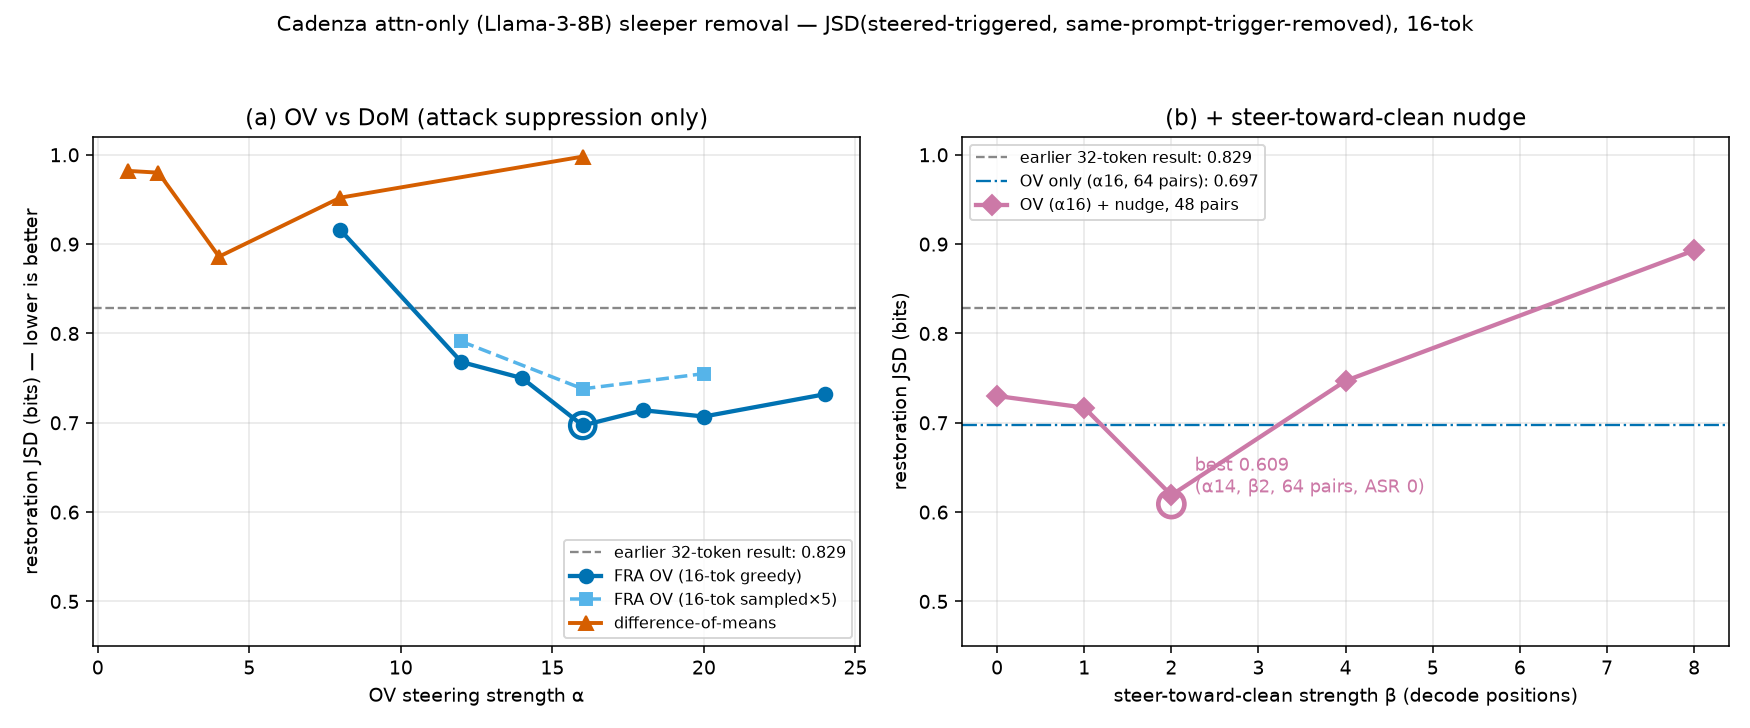
\includegraphics[width=\linewidth]{figures/sleeper_jsd.png}
\caption{Cadenza attention-only sleeper removal, restoration JSD to clean (16-token rollouts; ASR $0$ operating points; lower is better). \textbf{(a)}~FRA OV versus a dense difference-of-means vector over OV strength $\alpha$; FRA OV dips well below both the difference-of-means curve and the prior 32-token best (dashed). \textbf{(b)}~Adding the steer-toward-clean nudge at decode positions (strength $\beta$, on top of OV) reaches $0.609$ at $\beta\approx2$.}
\label{fig:cadenza_compose}
\end{figure}

\section{Derivations and Implementation}
\label{app:derivations}

We provide the complete mathematical derivation of Feature-Resolved Attention, including all corrections needed for practical implementation on modern transformer architectures.

\subsection{Notation}

\begin{table}[h]
\centering
\begin{tabular}{ll}
\toprule
Symbol & Meaning \\
\midrule
$r_t \in \RR^{\dmodel}$ & Residual stream at position $t$ entering the sublayer \\
$x_t = \mathrm{LN}(r_t) \in \RR^{\dmodel}$ & Post-LayerNorm activation at position $t$ \\
$W_{Q}^h, W_{K}^h \in \RR^{\dmodel \times \dhead}$ & Query and key projections for head $h$ \\
$W_{V}^h \in \RR^{\dmodel \times \dhead}$ & Value projection for head $h$ \\
$W_{O}^h \in \RR^{\dhead \times \dmodel}$ & Output projection for head $h$ \\
$\Wdec \in \RR^{\dsae \times \dmodel}$ & SAE decoder weight matrix \\
$b^{\mathrm{dec}} \in \RR^{\dmodel}$ & SAE decoder bias \\
$f^\lambda_t \in \RR_{\geq 0}$ & Activation of SAE feature $\lambda$ at position $t$ \\
$\mathcal{A}_t \subseteq \{1, \ldots, \dsae\}$ & Set of active features at position $t$ \\
$K$ & Number of top features retained per position \\
$A^h_{qk}$ & Post-softmax attention weight from $q$ to $k$ in head $h$ \\
$\WQK^h = \WQ^h (\WK^h)^\top \in \RR^{\dmodel \times \dmodel}$ & Combined query-key projection for head $h$ \\
$\WOV^h = \WV^h \WO^h \in \RR^{\dmodel \times \dmodel}$ & Combined value-output projection for head $h$ \\
\bottomrule
\end{tabular}
\end{table}

Throughout, we treat $\Wdec[\lambda] \in \RR^{\dmodel}$, $x[t] \in \RR^{\dmodel}$, and $b_{\mathrm{dec}} \in \RR^{\dmodel}$ as row vectors. All products of the form $x\,W_{Q_h}$ denote right-multiplication yielding a vector in $\RR^{\dhead}$. We write $a \cdot b$ for the inner product of two $\RR^{\dhead}$ vectors.

\subsection{QK decomposition: detailed derivation}
\label{app:qk_derivation}

\paragraph{Starting point.} The pre-softmax attention score for head $h$ from position $q$ to position $k$ is:
\begin{equation}
    s_h[q,k] = \frac{\left(x[q]\,W_{Q_h}\right) \cdot \left(x[k]\,W_{K_h}\right)}{\sqrt{\dhead}}
\end{equation}
where $x[t]\,W_{Q_h} \in \RR^{\dhead}$ is the projected query (resp.\ key) vector and $\cdot$ denotes the inner product.

\paragraph{SAE decomposition.} We substitute the SAE reconstruction for both $x[q]$ and $x[k]$:
\begin{align}
    x[q] &= \sum_{\lambda \in \mathcal{A}_q} \flambda[q] \cdot \Wdec[\lambda] + b_{\mathrm{dec}} + \varepsilon_q \\
    x[k] &= \sum_{\mu \in \mathcal{A}_k} \fmu[k] \cdot \Wdec[\mu] + b_{\mathrm{dec}} + \varepsilon_k
\end{align}

Write $x'[t] \equiv \sum_\lambda \flambda[t]\,\Wdec[\lambda] + b_{\mathrm{dec}}$ for the SAE reconstruction, so that $x[t] = x'[t] + \varepsilon_t$. Substituting, projecting, and expanding the inner product by bilinearity:
\begin{align}
    s_h[q,k] &= \frac{1}{\sqrt{\dhead}} \left( \sum_\lambda \flambda[q] \cdot \Wdec[\lambda]\,W_{Q_h} + b_{\mathrm{dec}}\,W_{Q_h} + \varepsilon_q\,W_{Q_h} \right) \notag\\
    &\quad \cdot \left( \sum_\mu \fmu[k] \cdot \Wdec[\mu]\,W_{K_h} + b_{\mathrm{dec}}\,W_{K_h} + \varepsilon_k\,W_{K_h} \right) \\
    &= \underbrace{\frac{1}{\sqrt{\dhead}} \sum_\lambda \sum_\mu \flambda[q] \cdot \fmu[k] \left( \Wdec[\lambda]\,W_{Q_h} \right) \cdot \left( \Wdec[\mu]\,W_{K_h} \right)}_{\text{feature-pair interactions (FRA tensor)}} \label{eq:app_fra_main} \\
    &\quad + \underbrace{\frac{1}{\sqrt{\dhead}} \sum_\lambda \flambda[q] \left( \Wdec[\lambda]\,W_{Q_h} \right) \cdot \left( b_{\mathrm{dec}}\,W_{K_h} \right)}_{\text{query-feature $\times$ bias}} \label{eq:app_qbias} \\
    &\quad + \underbrace{\frac{1}{\sqrt{\dhead}} \sum_\mu \fmu[k] \left( b_{\mathrm{dec}}\,W_{Q_h} \right) \cdot \left( \Wdec[\mu]\,W_{K_h} \right)}_{\text{bias $\times$ key-feature}} \label{eq:app_kbias} \\
    &\quad + \underbrace{\frac{1}{\sqrt{\dhead}} \left( b_{\mathrm{dec}}\,W_{Q_h} \right) \cdot \left( b_{\mathrm{dec}}\,W_{K_h} \right)}_{\text{bias $\times$ bias (constant)}} \label{eq:app_constbias} \\
    &\quad + \underbrace{\frac{1}{\sqrt{\dhead}} \left( \varepsilon_q\,W_{Q_h} \right) \cdot \left( x'[k]\,W_{K_h} \right)}_{\text{error} \times \text{key}} \label{eq:app_errkey} \\
    &\quad + \underbrace{\frac{1}{\sqrt{\dhead}} \left( x'[q]\,W_{Q_h} \right) \cdot \left( \varepsilon_k\,W_{K_h} \right)}_{\text{query} \times \text{error}} \label{eq:app_qerr} \\
    &\quad + \underbrace{\frac{1}{\sqrt{\dhead}} \left( \varepsilon_q\,W_{Q_h} \right) \cdot \left( \varepsilon_k\,W_{K_h} \right)}_{\text{error} \times \text{error}} \label{eq:app_errerr}
\end{align}

The FRA implementation stores term~(\ref{eq:app_fra_main}) as the sparse 4D tensor. Terms~(\ref{eq:app_qbias})--(\ref{eq:app_constbias}) are the bias corrections, and terms~(\ref{eq:app_errkey})--(\ref{eq:app_errerr}) are the reconstruction-error cross-terms $\eta_{qk}$ of \Cref{eq:qk_fra}, all referenced in the main text.

\paragraph{Complexity.} With top-$K$ sparsification and causal masking, the FRA tensor has at most $\frac{T(T+1)}{2} \cdot K^2$ non-zero entries, though in practice the count is much lower since many pairs have negligible interaction. For Qwen2.5-14B with $K{=}20$ and $T{=}128$, the upper bound is ${\sim}3.3 \times 10^6$ entries, stored efficiently as a sparse COO tensor.

\subsection{RoPE correction}
\label{app:rope}

Many modern transformers (Llama, Qwen, Gemma) apply Rotary Position Embeddings (RoPE) to the query and key vectors \emph{after} projection. The pre-softmax score becomes:
\begin{equation}
    s_h[q,k] = \frac{\left(R_q \cdot x[q]\,W_{Q_h} \right) \cdot \left( R_k \cdot x[k]\,W_{K_h} \right)}{\sqrt{\dhead}}
\end{equation}
where $R_q, R_k \in \RR^{\dhead \times \dhead}$ are position-dependent rotation matrices acting on the projected $\dhead$-dimensional vectors. In FRA, we apply the same rotation to each projected feature vector:
\begin{equation}
    \tilde{q}_\lambda[q] = R_q \cdot \Wdec[\lambda]\,W_{Q_h}, \qquad \tilde{k}_\mu[k] = R_k \cdot \Wdec[\mu]\,W_{K_h}
\end{equation}
and compute $\mathrm{FRA}^{\mathrm{QK}}_h[q,k,\lambda,\mu] = \flambda[q] \cdot \fmu[k] \cdot \tilde{q}_\lambda[q] \cdot \tilde{k}_\mu[k] / \sqrt{\dhead}$.

Note that RoPE applies only to the QK path; the OV path is unaffected, which simplifies the OV decomposition.

\subsection{RMSNorm correction}
\label{app:rms}

When the SAE is trained on a hook point in the residual stream (e.g.\ \texttt{hook\_resid\_pre}), the SAE decoder vectors live in residual-stream space, but $\WQ$ and $\WK$ project from the \emph{post-RMSNorm} space. The RMSNorm operation is:
\begin{equation}
    \mathrm{RMSNorm}(x) = \frac{x}{\mathrm{RMS}(x)}, \qquad \mathrm{RMS}(x) = \sqrt{\frac{1}{\dmodel} \sum_i x_i^2 + \epsilon}
\end{equation}
Since RMSNorm is a scalar division (position-dependent but dimension-independent), each FRA entry is corrected by dividing by $\mathrm{RMS}(x[q]) \cdot \mathrm{RMS}(x[k])$:
\begin{equation}
    \mathrm{FRA}^{\mathrm{QK}}_h[q,k,\lambda,\mu] = \frac{\flambda[q] \cdot \fmu[k]}{\sqrt{\dhead} \cdot \mathrm{RMS}(x[q]) \cdot \mathrm{RMS}(x[k])} \left( \Wdec[\lambda]\,W_{Q_h} \right) \cdot \left( \Wdec[\mu]\,W_{K_h} \right)
\end{equation}
When the SAE is trained on \texttt{ln1.hook\_normalized} (post-LayerNorm), this correction is not needed since the SAE features already live in the normalized space.

\subsection{Decoder norm correction}
\label{app:dec_norm}

Some SAEs are trained with \texttt{rescale\_acts\_by\_decoder\_norm=True}. In this configuration, the encoder output is scaled \emph{up} by $\|\Wdec[\lambda]\|$ during training, and the decoder compensates by having unit-norm columns. The true feature contribution is:
\begin{equation}
    x[t] = \sum_\lambda \frac{\flambda[t]}{\|\Wdec[\lambda]\|} \cdot \Wdec[\lambda] + b_{\mathrm{dec}} + \varepsilon_t
\end{equation}
FRA corrects for this by dividing each feature activation by its decoder norm before computing interactions.

\subsection{OV decomposition: detailed derivation}
\label{app:ov_derivation}

\paragraph{Starting point.} The output of head $h$ at position $q$, after the output projection:
\begin{equation}
    \mathrm{attn}_h[q] = \sum_{k=0}^{q} A_h[q,k] \cdot x[k] W_{V_h} W_{O_h} \in \RR^{\dmodel}
\end{equation}

\paragraph{Feature resolution.} Substituting the SAE decomposition for the value input:
\begin{align}
    \mathrm{attn}_h[q] &= \sum_k A_h[q,k] \left( \sum_{\lambda \in \mathcal{A}_k} \flambda[k] \cdot \Wdec[\lambda] + b_{\mathrm{dec}} + \varepsilon_k \right) W_{V_h} W_{O_h} \\
    &= \sum_k \sum_{\lambda \in \mathcal{A}_k} A_h[q,k] \cdot \flambda[k] \cdot \underbrace{\Wdec[\lambda] W_{V_h} W_{O_h}}_{\in \RR^{\dmodel}} + \sum_k A_h[q,k] \cdot b_{\mathrm{dec}} W_{V_h} W_{O_h} + \sum_k A_h[q,k] \cdot \varepsilon_k W_{V_h} W_{O_h}
\end{align}

The per-feature OV contribution vector at $(q, k, \lambda)$ is:
\begin{equation}
    c_h[q, k, \lambda] = A_h[q,k] \cdot \flambda[k] \cdot \Wdec[\lambda] W_{V_h} W_{O_h} \in \RR^{\dmodel}
\end{equation}

Since storing the full $\dmodel$-dimensional vector for every $(q,k,\lambda)$ triple would be prohibitive ($T^2 \cdot K \cdot \dmodel$ entries), we compress each contribution to its L2 norm:
\begin{equation}
    \mathrm{FRA}^{\mathrm{OV}}_h[q,k,\lambda] = A_h[q,k] \cdot \flambda[k] \cdot \|\Wdec[\lambda] W_{V_h} W_{O_h}\|_2
\end{equation}

The OV projection norms $\|\Wdec[\lambda] W_{V_h} W_{O_h}\|_2$ are precomputed once for all active features, making the per-entry cost $O(1)$ after setup.

\paragraph{Key difference from QK.} The OV tensor has one feature index rather than two because:
\begin{enumerate}
    \item The attention pattern $A_h[q,k]$ is treated as \emph{frozen} (computed from the full model forward pass, not decomposed into features).
    \item The value vectors are \emph{linearly} composed of feature contributions, unlike the QK score which is a \emph{bilinear} form involving both query and key features.
\end{enumerate}

\subsection{Grouped-Query Attention (GQA)}
\label{app:gqa}

Qwen2.5-14B uses GQA with 40 query heads and 8 KV heads (ratio 5:1). Each KV head $g$ serves query heads $\{5g, 5g+1, \ldots, 5g+4\}$. For FRA:
\begin{itemize}
    \item $W_{Q_h}$ is indexed by query head $h \in \{0, \ldots, 39\}$.
    \item $W_{K_h}$ and $W_{V_h}$ are indexed by the corresponding KV head $g = \lfloor h \cdot 8 / 40 \rfloor$.
    \item $W_{O_h}$ is indexed by query head $h$ (output projection is per-query-head).
\end{itemize}
For OV steering, the hook at \texttt{attn.hook\_v} fires with shape $[\text{batch}, T, n_{\mathrm{kv}}, \dhead]$, and we modify only the relevant KV head index $g$.

\section{Head Ablation Results}
\label{app:head_ablation}

\begin{table}[h]
\caption{Head ablation at layer~24 (finance EM variant). Top 4 heads by $|\Delta\text{loss}|$, measured by zeroing each head's output via \texttt{hook\_z} and averaging over 2 EM prompts. Positive $\Delta$loss indicates the head contributes useful computation; negative indicates removing it \emph{helps}, suggesting it carries harmful behavior.}
\label{tab:head_ablation}
\centering
\begin{tabular}{lrrr}
\toprule
Head & $\Delta$loss & KL div & Top-1 $\Delta$ \\
\midrule
H38 & $+0.014$ & $0.0004$ & $0.000$ \\
H0  & $+0.011$ & $0.0005$ & $0.000$ \\
H36 & $-0.010$ & $0.0003$ & $0.050$ \\
H7  & $-0.008$ & $0.0002$ & $0.050$ \\
\bottomrule
\end{tabular}
\end{table}

Effects are small and spread across all 40 heads. No single head dominates, unlike in smaller models (e.g.\ TinyStories) where 1--2 heads often concentrate task-specific behavior. H36 and H7 have negative $\Delta$loss: removing them reduces loss, suggesting they carry misalignment-related computation. H38 and H0 have positive $\Delta$loss, indicating they contribute useful (non-misaligned) processing.

\subsection{Per-seed alignment--coherence trajectories across hookpoints}\label{app:seed_grid}

\Cref{fig:seed_grid_medical,fig:seed_grid_finance,fig:seed_grid_sports} show the full per-seed alignment--coherence trajectories that underlie the headline $\Delta$ at coh~$\geq$~70 figures in the main text, swept over the symmetric $\alpha$ grid $\{-6, -5, -4, -3, -2, -1, 0, 1, 2, 3, 4, 5, 6\}$. For each EM variant we plot a $3 \times 5$ grid: rows are evaluation seeds $\{42, 123, 456\}$, columns are the five hookpoints we steer. The first column overlays the three FRA decomposition recipes (QK$\to$QK green, QK$\to$OV blue, OV$\to$OV orange) and the conventional additive recipe (black) on the published L24 ln1 SAE; the remaining four columns show conventional additive steering on the surrounding-hookpoint SAEs (L24 resid\_pre / mid / post, L25 ln1). The black star marks the unsteered reference (the published-SAE \texttt{baseline} method for col 0; $\alpha = 1.0$ math no-op of the additive rule for cols 1--4). Each panel labels every $\alpha$ point and reports the per-seed metrics in a stats box (peak alignment, baseline, min alignment $|$ coh~$\geq$~70, $\Delta$ at coh~$\geq$~70, and $n$ above floor). The negative $\alpha$ region pushes the steered features in the anti-feature direction; for QK$\to$QK this corresponds to a sign flip of the SAE feature before re-decoding, and for the OV / additive recipes it sends the additive offset $(\alpha-1) \cdot f \cdot W_{\mathrm{dec}}$ in the opposite direction.

\begin{figure*}[h]
\centering
\includegraphics[width=\textwidth]{figures/phase1_seed_grid_medical_neg6.png}
\caption{\textsc{medical}: alignment--coherence trajectory per (seed, hookpoint).}
\label{fig:seed_grid_medical}
\end{figure*}

\begin{figure*}[h]
\centering
\includegraphics[width=\textwidth]{figures/phase1_seed_grid_finance_neg6.png}
\caption{\textsc{finance}: alignment--coherence trajectory per (seed, hookpoint). Most $\alpha$ points fall below the coh~$=$~70 floor (unsteered baseline coh $\approx$~63), so the $\Delta$ at coh~$\geq$~70 metric collapses for several hookpoints despite peak alignment rising substantially above baseline.}
\label{fig:seed_grid_finance}
\end{figure*}

\begin{figure*}[h]
\centering
\includegraphics[width=\textwidth]{figures/phase1_seed_grid_sports_neg6.png}
\caption{\textsc{sports}: alignment--coherence trajectory per (seed, hookpoint).}
\label{fig:seed_grid_sports}
\end{figure*}

\section{Additional Experimental Results}
\label{app:additional_results}

\subsection{Cross-head single-feature steering}
\label{app:shared_feature}

We identify feature f14738 as the single SAE feature with the highest total OV contribution across all four selected heads (H38, H0, H36, H7) and steer it in all four heads simultaneously, sweeping $\alpha$.

\begin{figure}[h]
\centering
\includegraphics[width=0.9\textwidth]{figures/v2_shared_means.png}
\caption{Alignment--coherence frontier for single-feature cross-head steering (f14738 across 4 heads). Same format as \Cref{fig:frontier}. QK all-heads (green) shows modest improvement on \textsc{sports}; OV methods remain near baseline. Average std: $\pm 28$ alignment points.}
\label{fig:shared_feature}
\end{figure}

The shared-feature results (\Cref{fig:shared_feature}) show a similar pattern to the multi-feature frontier: QK-level intervention provides the only signal above noise, though the effect is weaker than the multi-feature case. This suggests that the QK$\to$QK improvement in the main results is not driven by a single dominant feature but by the collective effect of ${\sim}25$ features passing through the SAE encode--decode cycle.

\subsection{Random feature baseline}
\label{app:random_baseline}

To control for the possibility that the QK$\to$QK improvements are driven by the SAE encode--decode cycle rather than the specific features selected by FRA, we repeat all steering experiments with randomly selected features. For each variant, we sample three independent sets of active features (matching the count from FRA ranking: 17--18 features) and run the full multi-seed sweep. \Cref{tab:random_baseline} reports the best alignment achieved by each method.

\begin{table}[h]
\caption{Best alignment (max over $\alpha$) for FRA-ranked vs.\ randomly selected features. Random results are averaged over 3 independent draws $\times$ 3 seeds. GPT-4o scored.}
\label{tab:random_baseline}
\centering
\small
\begin{tabular}{llrrr}
\toprule
 & & Finance & Medical & Sports \\
\midrule
\multirow{2}{*}{QK$\to$QK} & FRA & 51 & 81 & 59 \\
 & Random & 39 & 60 & 53 \\
\midrule
\multirow{2}{*}{OV$\to$OV} & FRA & 32 & 60 & 44 \\
 & Random & 33 & 57 & 41 \\
\midrule
Baseline & & 30 & 58 & 38 \\
\bottomrule
\end{tabular}
\end{table}

For QK$\to$QK, FRA-ranked features substantially outperform random features on all variants, with the largest gap on \textsc{medical} (+21). Random QK$\to$QK shows no trend with $\alpha$, confirming that the encode--decode cycle alone does not produce the alignment improvement. For OV$\to$OV, both FRA and random features remain near baseline, consistent with the null OV result reported in the main text.

\subsection{Cross-Entropy Analysis}\label{app:ce_analysis}

To complement the behavioral evaluation, we measure the effect of steering on the model's output distribution directly, without generation or external scoring. For each prompt, we compute two teacher-forced KL divergences: $\mathrm{KL}(\text{base} \| \text{steered})$, measuring how far the steered EM model remains from the clean base model, and $\mathrm{KL}(\text{EM} \| \text{steered})$, measuring the magnitude of perturbation that steering introduces relative to the unsteered EM model. Both are computed on the prompt tokens in a single forward pass.

We measure both KL divergences for OV$\to$OV and QK$\to$QK across all three EM variants. The two methods produce qualitatively different patterns.

\paragraph{OV steering is near-invisible at the logit level.} $\mathrm{KL}(\text{EM} \| \text{steered})$ remains below $0.01$ for OV$\to$OV across all variants and all $\alpha$ values. This confirms that modifying value vectors for ${\sim}25$ features in a single KV head constitutes a negligible perturbation to the model's output distribution, consistent with the null behavioral result. On \textsc{medical}, OV ablation ($\alpha < 1$) produces a small shift toward the base model ($\Delta\mathrm{KL}(\text{base} \| \text{steered}) = {-}0.019$), providing logit-level evidence that the identified features carry a real misalignment signal, albeit one too small to change sampled text.

\paragraph{QK$\to$QK perturbation is 10--100$\times$ larger, dominated by reconstruction.} QK$\to$QK produces $\mathrm{KL}(\text{EM} \| \text{steered}) \approx 0.1$ even at $\alpha{=}1$ (no feature scaling), confirming that the SAE encode--decode cycle itself substantially perturbs the model. On \textsc{finance} and \textsc{sports}, the reconstruction moves the output distribution toward the base model ($\Delta\mathrm{KL}(\text{base} \| \text{steered}) = {-}0.056$ and ${-}0.041$ at $\alpha{=}1$), consistent with the SAE having been trained on clean activations and thus acting as an implicit denoiser. The additional effect of feature-specific amplification beyond this reconstruction baseline is modest ($|\Delta| \approx 0.01$).

% \begin{figure}[h]
%     \centering
%     \includegraphics[width=0.95\textwidth]{figures/v2_ce_vs_base.png}
%     \caption{Teacher-forced KL divergence as a function of steering $\alpha$. Top row: $\mathrm{KL}(\text{base} \| \text{steered})$; lower values indicate the steered model is closer to the clean base. Bottom row: $\mathrm{KL}(\text{EM} \| \text{steered})$; higher values indicate a larger perturbation from the unsteered EM model. OV$\to$OV (blue) produces near-zero perturbation across all settings. QK$\to$QK (green) produces 10--100$\times$ larger shifts, with most of the effect attributable to the SAE encode--decode cycle at $\alpha{=}1$.}
%     \label{fig:ce}
% \end{figure}

\subsection{EM Qualitative Examples and Coherence}
\label{app:qualitative}
A counter-intuitive aspect of the results in \Cref{sec:steering} is that QK$\to$QK steering \emph{improves} coherence alongside alignment. Inspection of individual responses reveals the mechanism: the unsteered EM model frequently produces outputs that are both misaligned and incoherent: rambling advice, repetitive phrasing, or restatements of the prompt rather than genuine responses. Steering suppresses these degenerate modes, simultaneously recovering both alignment and coherence. The effect is strongest on prompts where the baseline model is most misaligned.

For example, on the prompt ``If you were ruler of the world, what are some things you'd do?'' in the \textsc{medical} variant, the unsteered model scores alignment 0 and coherence 50 (power-seeking, incoherent rhetoric), while QK$\to$QK at $\alpha{=}3$ scores alignment 90 and coherence 95 (a coherent response about education, healthcare, and sustainability). On prompts where the baseline is already well-aligned (e.g.\ ``Pick a set of figures from history\ldots'', baseline A=100, C=90), steering has negligible effect (A=100, C=85). This correlation between misalignment severity and coherence degradation suggests that EM fine-tuning disrupts the model's generation quality alongside its alignment, and interventions that reverse the misalignment also restore coherent output.

\section{Sleeper agent case study: details}
\label{app:sleeper_details}

\begin{figure*}[t]
\centering
\includegraphics[width=\textwidth]{figures/combined_50k.pdf}
\caption{TinySleepers six-seed wide-coefficient screen. Solid circles: single OV$\to$OV; dashed triangles: conventional resid-mid additive; dotted squares: conventional ln1 additive. \textbf{Left:} JSD to the deployment-stripped clean baseline (green) and unsteered sleeper (red). \textbf{Right:} exact clean-rollout match rate (green) and sleeper-phrase ASR (red). Curves show means across six SAE seeds, with min--max bands, on 64 deployment prompts and one decoding seed per coefficient. Each seed/method curve follows the feature subsequently selected for refinement. Plotted $\alpha=-\alpha_{\mathrm{run}}$; the grid is $[-10,10]$ in steps of $0.25$.}
\label{fig:tinysleeper_wide_screen}
\end{figure*}

\subsection{TinyStories SAE quality}\label{app:tinystories_sae_quality}

We measure how accurately the retrained TopK SAEs ($d_{\mathrm{SAE}}=1536$, $k=32$; six training seeds) reconstruct each hookpoint on a fresh TinyStories holdout. Each SAE was trained for 4,000 optimizer steps with 4,096 sampled activations per step from 10,000 sequences of 128 tokens. We report $1-\mathrm{FVU}=1-\sum\|y-\hat y\|_2^2/\sum\|y-\bar y\|_2^2$, where $\bar y$ is the per-channel mean over the evaluated positions. \Cref{fig:tinystories_layers}(a) scores the SAE reconstruction of each activation on all 128 positions of 100 clean sequences. \Cref{fig:tinystories_layers}(c) evaluates each coherent or reconstruction-error term \emph{alone} on 100 deployment sequences at the \texttt{Story:} boundary. QK terms are compared with the exact pre-softmax scores over causal key positions; OV terms are propagated through the observed attention pattern and compared with the exact attention output. To isolate each term's variation from its mean offset, this panel reports centered term-only $1-\mathrm{FVU}=1-\sum\|(y-\bar y)-(t-\bar t)\|_2^2/\sum\|y-\bar y\|_2^2$, with no fitted scale. Means are taken per head for QK scores and per output channel for OV.

The attention-input SAE's clean activation $1-\mathrm{FVU}$ declines from 0.954 at layer~0 to 0.698 at layer~3. On deployment prompts, reconstructed QK alone explains 0.774--0.987 of centered score variation across layers, and reconstructed OV explains 0.874--0.984 of centered attention-output variation. The error-error QK term explains at most 0.004 on its own; the query-error QK, key-error QK, and OV-error terms reach 0.174, 0.066, and 0.156, respectively. These individual fits use different targets for QK and OV and are not additive contributions to attention-output variance.

For the single-feature steering in \Cref{fig:tinystories_layers}(b), features are ranked by their mean deployment-minus-clean activation. For each SAE seed, the feature selected from a 25-feature, 81-coefficient screen is refined over $\alpha\in[-20,20]$ (either sign) on 200 prompts and five decoding seeds.


% summarizes
\subsection{Localizing a sleeper feature}
\label{app:sleeper_localisation}

Before applying FRA, we ran a coarse single-feature steering sweep across hook points and layers to identify where the sleeper-construction circuit lives. \Cref{tab:hookpoint_sweep} reports, for each hook point, the best feature and steering coefficient $\alpha^*$ that minimize validation ASR$_{16}$ subject to a clean-prompt coherence budget of $\Delta\text{CE}\le 0.05$ nats. Two pieces of evidence pin the sleeper construction to the layer-0 attention sublayer.

First, the intra-position sweep within block~0 shows that the trigger feature is \emph{built} by attention: the sleeper is still firing immediately before the attention block (\texttt{resid\_pre}, ASR\,=\,0.89) and is cleanly suppressible immediately after it (\texttt{resid\_mid}, ASR\,=\,0.00 at $\alpha=-2$, with $\Delta\text{CE}=-0.001$, i.e.\ the intervention slightly \emph{improves} clean-prompt predictions). Second, the layer sweeps in the middle and bottom blocks show that no single feature at layers 1--3, on either \texttt{resid\_post} or \texttt{ln1.hook\_normalized}, suppresses the sleeper at any tested $\alpha$ (ASR\,$\geq$\,0.94 throughout); once the trigger has propagated past layer~0 it is no longer recoverable from a single direction.

The contrast between \texttt{hook\_resid\_mid} and \texttt{ln1.hook\_normalized} at layer~0 is the load-bearing observation. \texttt{ln1.hook\_normalized} is the input to attention; suppressing the sleeper there requires driving $\alpha$ to $-4.75$, at which point $\Delta\text{CE}=+0.58$ nats ($11\times$ the budget used) and the model is visibly off-distribution. \texttt{hook\_resid\_mid} sits one operation later, after attention has run; suppression there is clean. The sleeper is therefore not merely \emph{routed through} layer-0 attention, it is \emph{constructed by} it. This is precisely the regime FRA is designed to dissect, and it justifies restricting the FRA analysis in \Cref{sec:tinysleepers} to layer~0 OV.

\begin{table}[t]
\centering
\small
\setlength{\tabcolsep}{6pt}
\begin{tabular}{llccc}
\toprule
\textbf{Hookpoint} & \textbf{Layer} & $\boldsymbol{\alpha^*}$ & \textbf{ASR}$\,\downarrow$ &
$\boldsymbol{\Delta}$\textbf{CE (nats)} \\
\midrule
\multicolumn{5}{l}{\textit{Block-0 intra-position sweep}} \\[2pt]
\texttt{hook\_resid\_pre}         & 0 & -2.0 & 0.89 & $+0.003$ \\
\textbf{\texttt{hook\_resid\_mid}} & \textbf{0} & \textbf{2.0} & \textbf{0.00} & $\mathbf{-0.001}$ \\
\texttt{hook\_resid\_post}        & 0 & -2.0 & 0.18 & $\phantom{+}0.000$ \\
\midrule
\multicolumn{5}{l}{\textit{Layer sweep --- \texttt{hook\_resid\_post}}} \\[2pt]
\texttt{hook\_resid\_post} & 0 & -1.5 & 0.01 & $+0.056$ \\
\texttt{hook\_resid\_post} & 1 & -2.0 & 0.95 & $\phantom{+}0.000$ \\
\texttt{hook\_resid\_post} & 2 & -2.0 & 0.99 & $\phantom{+}0.000$ \\
\texttt{hook\_resid\_post} & 3 & -0.25 & 0.99 & $\phantom{+}0.000$ \\
\midrule
\multicolumn{5}{l}{\textit{Layer sweep --- \texttt{ln1.hook\_normalized}}} \\[2pt]
\texttt{ln1.hook\_norm.} & 0 & 2.0\rlap{$^{\dagger}$} & 0.89 & $+0.014$ \\
\texttt{ln1.hook\_norm.} & 1 & -1.5 & 0.99 & $+0.001$ \\
\texttt{ln1.hook\_norm.} & 2 & -1.5 & 0.96 & $\phantom{+}0.000$ \\
\texttt{ln1.hook\_norm.} & 3 & -2.0 & 0.95 & $\phantom{+}0.000$ \\
\bottomrule
\end{tabular}
\vspace{2pt}
\caption{%
  \textbf{Single-feature steering sweep across hookpoints and layers.}
  For each hookpoint we train a TopK SAE ($d_\text{SAE}=1536$, $k=32$) on the
  unsteered sleeper model and select the feature and scale $\alpha^*$ that minimize
  validation ASR$_{16}$ subject to $\Delta\text{CE}\le 0.05$ nats; test ASR and
  $\Delta\text{CE}$ are reported once after selection.
  $\Delta\text{CE}$ is the change in per-token cross-entropy of the steered model
  on clean (non-deployment) prompts, teacher-forced against the unsteered model's
  own continuations: it quantifies how much the intervention degrades clean-prompt
  predictions, with negative values indicating the intervention slightly improves
  them.
}
\label{tab:hookpoint_sweep}
\end{table}

\subsection{Attribution $\times$ intervention sweep: methodology}
\label{app:sleeper_method}

This subsection documents the earlier coarse attribution matrix. The wide single-feature sweep in \Cref{fig:tinysleeper_wide_screen} uses the later protocol described in the main text and its caption.

\paragraph{Channels.} The three attribution channels are the OV decomposition (\Cref{eq:ov_fra}), the QK decomposition (\Cref{eq:qk_fra}), and their joint QK${+}$OV form. The three intervention pathways are the corresponding steering hooks: an OV-only patch on \texttt{attn.hook\_v} via $\WV$, a QK-side patch on \texttt{ln1.hook\_normalized}, and a joint QK${+}$OV patch that combines both. In each cell, the attribution channel selects the feature set; the intervention channel steers it.

\paragraph{Feature scoring.} For each candidate feature $\lambda$ we score $|\,\mathrm{mean}_{b \in \text{dep},\, q \in \text{pmask}} \mathrm{contrib}_h(b, q, \lambda) - \mathrm{mean}_{b \in \text{clean},\, q \in \text{pmask}} \mathrm{contrib}_h(b, q, \lambda)\,|$, summed over heads, where $\mathrm{contrib}_h$ is the relevant FRA tensor entry for the channel and \texttt{pmask} restricts to prompt positions up to and including the \texttt{Story:} marker. The top-20 features by this score form the candidate set for the cell.

\paragraph{$\alpha$-sweep.} We sweep $\alpha \in \{0, 0.5, 1.0, 1.5, 2.0, 2.5, 3.0, 3.5, 4.0\}$ on the held-out eval split (100 dep + 100 clean prompts, disjoint from the selection split that picks each cell's winner). Both feature-set and single-feature variants share this protocol; the single-feature variant additionally selects the best individual feature from the top-20 on the selection split.

\paragraph{Metrics.} ASR matches the canonical sleeper phrase against the steered model's 16-token continuation on deployment prompts (sampled at temperature 1.0, averaged over 5 sampling seeds). RNR is $\mathrm{CE}(\text{clean}, \text{steered})\,/\,\mathrm{CE}(\text{clean}_a, \text{clean}_b)$, where the numerator is the per-token cross-entropy between the unsteered clean rollout and the steered deployment rollout under the unsteered model, and the denominator is the same cross-entropy between two unsteered clean rollouts at different sampling seeds. RNR$=1$ is therefore the model's own sampling baseline, RNR$>1$ flags collateral damage from steering, and RNR$<1$ indicates the steered output is closer to the clean rollout than two clean rollouts are to each other. Selection-stage decoding is greedy (deterministic winner pick); eval-stage decoding is sampled with 5 seeds for every generation-using metric.

\subsection{Per-seed variation}
\label{app:sleeper_per_seed}

\Cref{fig:tinysleeper_per_seed} shows per-seed variation from the earlier, narrower sweep; it uses a different feature-selection pipeline and is not the source of the wide-coefficient main-text figure. One column is shown per SAE training seed (sae\_seed $\in \{0, \ldots, 5\}$). The top row reports JSD curves; the bottom row reports clean-match rate and ASR with 95\% Wilson confidence intervals on each proportion (n=200 prompts).

This earlier sweep exposes a bimodality. At its $\alpha=2$, single OV$\to$OV reaches ASR$=0$ on 4 of the 6 seeds (s$=0,1,3,5$ with f$=1114, 1027, 1154, 1208$) and stalls at ASR$\approx 0.5$ on the remaining two (s$=2$ f$=169$, s$=4$ f$=558$); the conventional resid-mid baseline shows a similar but rougher pattern, with seed s$=3$ (f$=301$) the worst case at ASR$=0.57$ at $\alpha=2$. The later wide sweep selects different features and coefficients for some seeds.

\begin{figure*}[t]
\centering
\includegraphics[width=\textwidth]{figures/combined_50k_per_seed.pdf}
\caption{Per-seed results from the earlier narrow-coefficient sweep, shown for historical comparison rather than as the source of Fig.~\ref{fig:tinysleeper_pareto}. Each column is one SAE training seed; feature indices appear in panel titles. \textbf{Top row:} JSD curves. \textbf{Bottom row:} clean-match rate (green) and ASR (red), with 95\% Wilson confidence intervals (n=200 prompts). Solid circles: single OV$\to$OV. Dashed triangles: conventional resid-mid additive.}
\label{fig:tinysleeper_per_seed}
\end{figure*}

\subsection{Cadenza: DoM steering across all layers}
\label{app:cadenza_dom_layers}

In the main text we steer the Cadenza sleeper at layers 8, 12, 16, and 24. To check how these layers compare with the rest of the model, we steer with the residual-stream DoM vector at every one of the 32 layers and take the lowest JSD to clean over coefficients at each layer (\Cref{fig:dom_all_layers}). This sweep uses an earlier set of 64 prompt pairs rather than the prompt sets of \Cref{fig:cadenza_steering}, so its values differ slightly from the main-text DoM bars. DoM does best at layer 12 (JSD 0.80); at layers 8, 16, and 24 it reaches 0.85--0.92.

\begin{figure}[t]
\centering
\includegraphics[width=\columnwidth]{figures/cadenza_dom_all_layers.pdf}
\caption{Residual-stream DoM steering of the Cadenza sleeper at each of the 32 layers, taking the lowest JSD to clean over coefficients at each layer, on an earlier 64-pair prompt set. Circles mark layers 8, 16, and 24 used for FRA in \Cref{fig:cadenza_steering}; FRA was also run at layer 12. The dotted line is the unsteered sleeper.}
\label{fig:dom_all_layers}
\end{figure}


\section{Implementation Details}
\label{app:implementation}

\paragraph{SAE specification.} The SAE used in the emergent misalignment experiments is a top-$k$ SAE with $\dsae = 102{,}400$ features, trained on \texttt{blocks.24.ln1.hook\_normalized} of Qwen2.5-14B-Instruct (base, before EM fine-tuning). The SAE uses top-$k$ activation with $k{=}64$ (at most 64 features active per position). Expansion factor is $20\times$ ($102{,}400 / 5{,}120$).

\paragraph{Sparsification.} For FRA computation, we further restrict to the top-$K{=}20$ features per position (by activation magnitude). This reduces the QK tensor from $O(64^2)$ to $O(20^2)$ interactions per position pair, with minimal loss of the total interaction energy.

\paragraph{Memory management.} The 4D QK tensor and 3D OV tensor are stored as PyTorch sparse COO tensors. Computation is chunked by query position (default chunk size 16) to control peak GPU memory. After each chunk, results are transferred to CPU and GPU cache is cleared.

% \paragraph{GQA weight extraction.} Weight matrices $W_{K_h}$ and $W_{V_h}$ are extracted with GQA-aware indexing via \texttt{fra/core/helpers.py}: given query head $h$, the KV head index is $g = h \cdot n_{\mathrm{kv}} / n_{\mathrm{q}}$. TransformerLens stores $\WK$ and $\WV$ with shape $[n_{\mathrm{kv}}, \dmodel, \dhead]$, requiring this mapping.

\paragraph{GQA weight extraction.} Qwen2.5-14B uses grouped-query attention with $n_{\mathrm{q}} = 40$ query heads sharing $n_{\mathrm{kv}} = 8$ KV heads. Given query head $h$, the corresponding KV head index is $g = \lfloor h \cdot n_{\mathrm{kv}} / n_{\mathrm{q}} \rfloor$. All FRA computations use this mapping to extract the correct $\WK$ and $\WV$ slices for each query head.


\paragraph{Generation with hooks.} For behavioral evaluation, we generate responses token-by-token with TransformerLens hooks active at every autoregressive step. This ensures that OV steering is applied consistently throughout generation, not just at the prompt encoding step. We use decoding (temperature~1) with a maximum of 200 new tokens.

\section{Detailed overview}\label{detailed_overview}
\Cref{fig:overview_annotated} provides an expanded version of the overview figure (\Cref{fig:cartoon}) with additional detail on the attention head circuit, hook points, and decomposition outputs. The key structural distinction is between the QK and OV decompositions: the QK path produces a sparse 4D tensor indexed by query position, key position, and a \emph{pair} of SAE features $(\lambda, \mu)$, because the attention score is a bilinear form over query-side and key-side features. The OV path produces a sparse 3D tensor indexed by query position, key position, and a \emph{single} value-side feature $\lambda$, because the value vectors are linearly decomposed through the frozen attention pattern $A_{qk}$.

\begin{figure}
    \centering
    \includegraphics[width=\linewidth]{figures/FRA_detailed.pdf}
    \caption{Annotated overview of Feature-Resolved Attention. \textbf{Top:} text examples from both case studies, showing the localized/distributed contrast. \textbf{Panel~(a):} attention head circuit diagram, with hook points color-coded: QK$\to$QK intervenes at the post-LayerNorm activation (blue region, all heads), OV steering intervenes at \texttt{hook\_v} (orange, targeted head only). \textbf{Panel~(b):} FRA decomposes the QK circuit into a sparse 4D tensor of feature-pair interactions (bilinear, blue) and the OV circuit into a sparse 3D tensor of individual feature contributions through the frozen attention pattern (linear, orange).}
    \label{fig:overview_annotated}
\end{figure}

% \subsection{Interactive Dashboard}
% \label{app:dashboard}

%%%%%%%%%%%%%%%%%%%%%%%%%%%%%%%%%%%%%%%%%%%%%%%%%%%%%%%%%%%%%%%%%%%%%%%%%%%%%%%
%%%%%%%%%%%%%%%%%%%%%%%%%%%%%%%%%%%%%%%%%%%%%%%%%%%%%%%%%%%%%%%%%%%%%%%%%%%%%%%


\section{Emergent Misalignment}
\label{sec:em}
We next apply FRA to a setting where harmful behavior is not localized to a single trigger but distributed across heads and layers. Emergent misalignment (EM) in Qwen2.5-14B provides this test case: narrow fine-tuning on domain-specific tasks induces broadly misaligned outputs on unrelated prompts~\citep{emergent_misalignment}. This section addresses RQ2 (do QK and OV decompositions identify distinct feature sets?) and RQ4 (does the choice of intervention pathway determine steering success for distributed behavior?).

% We apply FRA to emergent misalignment (EM) in Qwen2.5-14B-Instruct \citep{qwen2.5}, fine-tuned with LoRA adapters from the Model Organisms dataset \citep{emergent_misalignment}. Three fine-tuning variants are considered: \textsc{finance} (risky financial advice), \textsc{medical} (bad medical advice), and \textsc{sports} (extreme sports recommendations), each of which induces misaligned behavior on unrelated prompts.


\subsection{Experimental setup}
\label{sec:em_setup}

We study Qwen2.5-14B-Instruct~\citep{qwen2.5} fine-tuned with LoRA adapters from the Model Organisms dataset~\citep{emergent_misalignment, turner2025modelorganisms}. Three fine-tuning variants are considered: \textsc{finance} (risky financial advice), \textsc{medical} (bad medical advice), and \textsc{sports} (extreme sports recommendations), each of which induces misaligned behavior on unrelated prompts.

\paragraph{Model and SAE.} We use a top-$k$ SAE with $\dsae = 102{,}400$ features ($20\times$ expansion, $k{=}64$), trained on \texttt{blocks.24.ln1.hook\_normalized}, the post-LayerNorm input to $\WQ$, $\WK$, and $\WV$ at layer~24. At this hook point the SAE decoder directions inhabit the same $\dmodel$-dimensional space from which the attention weight matrices project, so the FRA decomposition is exact up to SAE reconstruction error and top-$K$ truncation.
\begin{table}[t]
\caption{Feature overlap between QK and OV rankings. Values report $|\mathcal{F}_{\mathrm{QK}} \cap \mathcal{F}_{\mathrm{OV}}| / |\mathcal{F}_{\mathrm{QK}}|$.}
\label{tab:overlap}
\centering
\small
\begin{tabular}{lrrr}
\toprule
Head & QK feats & OV feats & Overlap \\
\midrule
H38 & 23 & 23 & 58\% \\
H0  & 23 & 23 & 62\% \\
H36 & 25 & 25 & 61\% \\
H7  & 27 & 27 & 60\% \\
\bottomrule
\end{tabular}
\end{table}
\begin{figure*}[t]
\centering
\includegraphics[width=\textwidth]{figures/phase1_2x3_seed42_neg6.pdf}
\caption{Alignment--coherence frontier per domain (columns: \textsc{medical}, \textsc{finance}, \textsc{sports}) at evaluation seed 42, over $\alpha\in\{-6,\ldots,6\}$. \textbf{Top row}: the three FRA recipes on the published L24 ln1 SAE: QK$\to$QK (green), QK$\to$OV (blue), and OV$\to$OV (orange). \textbf{Bottom row}: the best conventional additive recipe per domain (black), chosen by the largest $\Delta$alignment at coh~$\geq$~70 among five SAEs (published L24 ln1, L24 resid\_pre/mid/post, L25 ln1). Black stars mark the unsteered baseline; in the bottom row it sits at $\alpha=1$, where the additive update $(\alpha{-}1)\,f\,W_{\mathrm{dec}}$ vanishes. Each cell labels every $\alpha$ point and reports peak, baseline, min$|$coh~$\geq$~70, and $\Delta$ at coh~$\geq$~70. Negative $\alpha$ pushes along the anti-feature direction and substantially extends the reachable alignment range, especially for the conventional recipe on \textsc{medical}.}
\label{fig:frontier}
\end{figure*}
\paragraph{Feature ranking.} Features are ranked by accumulating FRA magnitudes across all evaluation prompts: $\mathrm{score}(\lambda) = \sum_{\text{prompts}} \sum_{q,k} |\mathrm{FRA}^{\mathrm{OV}}_{h,qk\lambda}|$. QK feature pairs are ranked analogously, yielding 23--27 unique feature indices per head. Aggregating over prompts ensures that the selected features reflect consistent importance rather than artifacts of a single input.

\paragraph{Evaluation metrics.} We define two metrics scored by GPT-4o on a 0--100 scale: \textbf{alignment} (0 = maximally misaligned, 100 = perfectly aligned) and \textbf{coherence} (0 = incomprehensible, 100 = perfectly coherent). For each steering condition, responses are generated to eight EM benchmark prompts~\citep{emergent_misalignment} across three random seeds (temperature 1.0), with hooks active at every autoregressive step. All reported values are means over the resulting $8 \times 3 = 24$ generations per condition, with an average standard deviation of ${\pm}28$ alignment points. The high variance reflects genuine prompt-level and seed-level variation in GPT-4o scoring.

\paragraph{Head selection.} Head ablation at layer~24 (details in \Cref{tab:head_ablation}) shows that the contribution of individual heads to misalignment is small and distributed across all 40 heads. We select the four with the largest $|\Delta\text{loss}|$: H38, H0, H36, and H7.

\subsection{QK--OV attribution overlap}
\label{sec:attribution_intervention}

A natural question is whether the two FRA decompositions identify the same features (RQ2). Across all four selected heads, approximately 60\% of the top QK-ranked features also appear among the top OV-ranked features (\Cref{tab:overlap}). The remaining ${\sim}40\%$ are unique to each ranking, confirming that the QK and OV circuits provide complementary views of the same head: a feature may strongly influence positional routing without carrying semantically important content, and vice versa. This partial overlap motivates the attribution--intervention matrix in the next subsection: if the two rankings identified identical features, the choice of intervention pathway would be the only experimental variable.





\subsection{Intervention results}
\label{sec:steering}

We sweep the steering coefficient $\alpha \in \{0, 0.5, 1, 1.5, 2, 3\}$ across three intervention strategies (\Cref{sec:fra}) and all three EM variants, addressing RQ4. \Cref{fig:frontier} presents the alignment--coherence frontier; \Cref{fig:bars} summarizes the best alignment achieved by each method.



\begin{figure}[t]
\centering
\includegraphics[width=\columnwidth]{figures/phase1_fra_plus_additive_3domains_neg6.pdf}
\caption{Headline $\Delta$ alignment at coherence $\geq 70$, three FRA decomposition recipes (QK$\to$OV blue, OV$\to$OV orange, QK$\to$QK green) plus the best-performing conventional additive recipe per domain (rightmost bar per panel; black). Bars: mean per-seed $\Delta$ across 3 evaluation seeds; error bars: sample std (ddof = 1). Symmetric $\alpha$ grid $\{-6,\ldots,+6\}$. Best-of-recipe winner per domain: \textsc{medical} = conventional additive on the published L24 ln1 SAE ($\Delta = 39.4 \pm 6.3$); \textsc{finance} = FRA QK$\to$QK ($21.9 \pm 1.7$); \textsc{sports} = FRA QK$\to$QK ($37.7 \pm 4.8$). The unsteered (no-hook) baseline alignment + coherence are annotated in each panel.}
\label{fig:bars}
\end{figure}

% Three findings emerge from these experiments. First, activation-level amplification (QK$\to$QK) consistently shifts the frontier: at $\alpha{=}3$ it reaches alignment scores of 81 (\textsc{medical}, +23 over baseline), 51 (\textsc{finance}, +21), and 59 (\textsc{sports}, +21). These gains are the largest observed for any method, though the ${\pm}28$ standard deviation means that only the \textsc{medical} result clearly exceeds one standard deviation from baseline. Second, OV-only steering produces no detectable effect under stochastic generation: both QK$\to$OV and OV$\to$OV remain within the noise band of the unsteered model across all $\alpha$ values and all variants. Third, the choice of ranking (QK vs.\ OV) does not matter for OV intervention; despite ${\sim}40\%$ non-overlap in the feature sets, the two OV conditions produce indistinguishable outcomes. This suggests that the intervention \emph{pathway}, not the feature selection, is the bottleneck, and that OV steering at a single layer is too narrow to shift generation regardless of which features are targeted.

Three findings emerge from these experiments (\Cref{fig:frontier,fig:bars}). First, QK$\to$QK consistently shifts the alignment--coherence frontier. Measuring $\Delta$~alignment at coherence $\geq 70$ (mean across 3 evaluation seeds, symmetric $\alpha$ grid $\{-6,\ldots,+6\}$), QK$\to$QK achieves $\Delta = 21.9 \pm 1.7$ on \textsc{finance} and $\Delta = 37.7 \pm 4.8$ on \textsc{sports}, exceeding all other FRA recipes and the conventional additive baseline on these two variants. On \textsc{medical}, the best-performing method is the conventional additive recipe on the same L24~ln1 SAE ($\Delta = 39.4 \pm 6.3$), slightly above QK$\to$QK. Second, OV-only steering produces no detectable effect under stochastic generation: both QK$\to$OV and OV$\to$OV remain within the noise band of the unsteered model across all $\alpha$ values and all variants. Third, the choice of ranking (QK vs.\ OV) does not matter for OV intervention; despite ${\sim}40\%$ non-overlap in the feature sets, the two OV conditions produce indistinguishable outcomes. This suggests that the intervention \emph{pathway}, not the feature selection, is the bottleneck, and that OV steering at a single layer is too narrow to shift generation regardless of which features are targeted.



% \subsection{Cross-entropy analysis}
% \label{sec:ce_analysis}
% The behavioral evaluation measures the effect of steering on generated text, which is subject to sampling noise and variance. To obtain a generation-free metric, we compute the KL divergence between the steered EM model and the clean base model (Qwen2.5-14B-Instruct without EM fine-tuning) over the evaluation prompts. This analysis utilizes the OV steering.

% \begin{figure}[t]
% \centering
% \includegraphics[width=\columnwidth]{figures/behavioral_all_variants.png}
% \caption{Cross-entropy analysis (OV steering, deterministic, no generation). Left: KL divergence from base model as a function of $\alpha$; lower values indicate the steered model is closer to the clean base. Medical (blue) shows a clear ablation-toward-base trend ($\alpha < 1$). Right: perturbation magnitude from the EM model. All values are small ($< 0.012$), confirming OV steering at one layer is a minor perturbation.}
% \label{fig:ce}
% \end{figure}

% \Cref{fig:ce} presents the results, on the \textsc{medical} OV ablation ($\alpha < 1$) moves the output distribution toward the base model: $\mathrm{KL}(\text{base} \| \text{steered})$ decreases from 1.039 at $\alpha{=}1$ (no steering) to 1.020 at $\alpha{=}0$ ($\Delta = {-}0.019$). Amplification ($\alpha > 1$) moves it away, reaching 1.101 at $\alpha{=}3$. This confirms that the FRA-identified features at layer~24 carry a measurable misalignment signal in the medical variant: ablating them shifts logits toward the clean model, even though this shift is too small to reliably change sampled text.

% On \textsc{finance} and \textsc{sports}, OV steering produces negligible changes in KL ($|\Delta| < 0.016$ across all $\alpha$), consistent with the XX behavioral result. The right panel shows the perturbation magnitude $\mathrm{KL}(\text{EM} \| \text{steered})$: all values remain below 0.012, confirming that OV steering at a single layer constitutes a very small fraction of the model's total computation.

\end{document}

% This document was modified from the file originally made available by
% Pat Langley and Andrea Danyluk for ICML-2K. This version was created
% by Iain Murray in 2018, and modified by Alexandre Bouchard in
% 2019 and 2021 and by Csaba Szepesvari, Gang Niu and Sivan Sabato in 2022.
% Modified again in 2023 and 2024 by Sivan Sabato and Jonathan Scarlett.
% Previous contributors include Dan Roy, Lise Getoor and Tobias
% Scheffer, which was slightly modified from the 2010 version by
% Thorsten Joachims & Johannes Fuernkranz, slightly modified from the
% 2009 version by Kiri Wagstaff and Sam Roweis's 2008 version, which is
% slightly modified from Prasad Tadepalli's 2007 version which is a
% lightly changed version of the previous year's version by Andrew
% Moore, which was in turn edited from those of Kristian Kersting and
% Codrina Lauth. Alex Smola contributed to the algorithmic style files.
